\documentclass[a4paper]{article} 
\addtolength{\hoffset}{-2.25cm}
\addtolength{\textwidth}{4.5cm}
\addtolength{\voffset}{-3.25cm}
\addtolength{\textheight}{5cm}
\setlength{\parskip}{0pt}
\setlength{\parindent}{0in}

\usepackage{blindtext} % Package to generate dummy text
\usepackage{charter} % Use the Charter font
\usepackage[utf8]{inputenc} % Use UTF-8 encoding
\usepackage{microtype} % Slightly tweak font spacing for aesthetics
\usepackage[english]{babel} % Language hyphenation and typographical rules
\usepackage{amsthm, amsmath, amssymb} % Mathematical typesetting
\usepackage{float} % Improved interface for floating objects
\usepackage[final, colorlinks = true, 
linkcolor = black, 
citecolor = black]{hyperref} % For hyperlinks in the PDF
\usepackage{graphicx, multicol} % Enhanced support for graphics
\usepackage{xcolor} % Driver-independent color extensions
\usepackage{marvosym, wasysym} % More symbols
\usepackage{rotating} % Rotation tools
\usepackage{subcaption}
\usepackage{wrapfig}
\usepackage[makeroom]{cancel}
\usepackage{censor} % Facilities for controlling restricted text
\newcommand{\note}[1]{\marginpar{\scriptsize \textcolor{red}{#1}}} % Enables comments in red on margin
\usepackage{bm}
\usepackage{blkarray}
\usepackage{enumitem}
\usepackage{pgfplots}
\usepackage{tikz}
\definecolor{colkeyword}{rgb}{0,0.4,0}
\definecolor{colname}{rgb}{0.4,0.4,0}
\definecolor{coltype}{rgb}{0.4,0,0.4}
\definecolor{coloperators}{rgb}{0,0,1.0}
\definecolor{colscopes}{rgb}{0.4,0,0}

\setcounter{tocdepth}{2}
% Title Page
\title{Summary Computer Vision 1}
\author{Phillip Lippe}


\begin{document}
\maketitle
\tableofcontents
\newpage

% \section{Introduction}
\subsection{Challenges in Computer Vision}
\begin{itemize}
	\item 
\end{itemize}
\section{Image formation}
\label{sec:img_formation}
\begin{itemize}
	\item To fully understand/analyze an image, we first have to examine how it was created (note that an image is a 2D representation of a 3D world)
	\item Various challenges occur in CV 
	\begin{figure}[ht!]
		\centering
		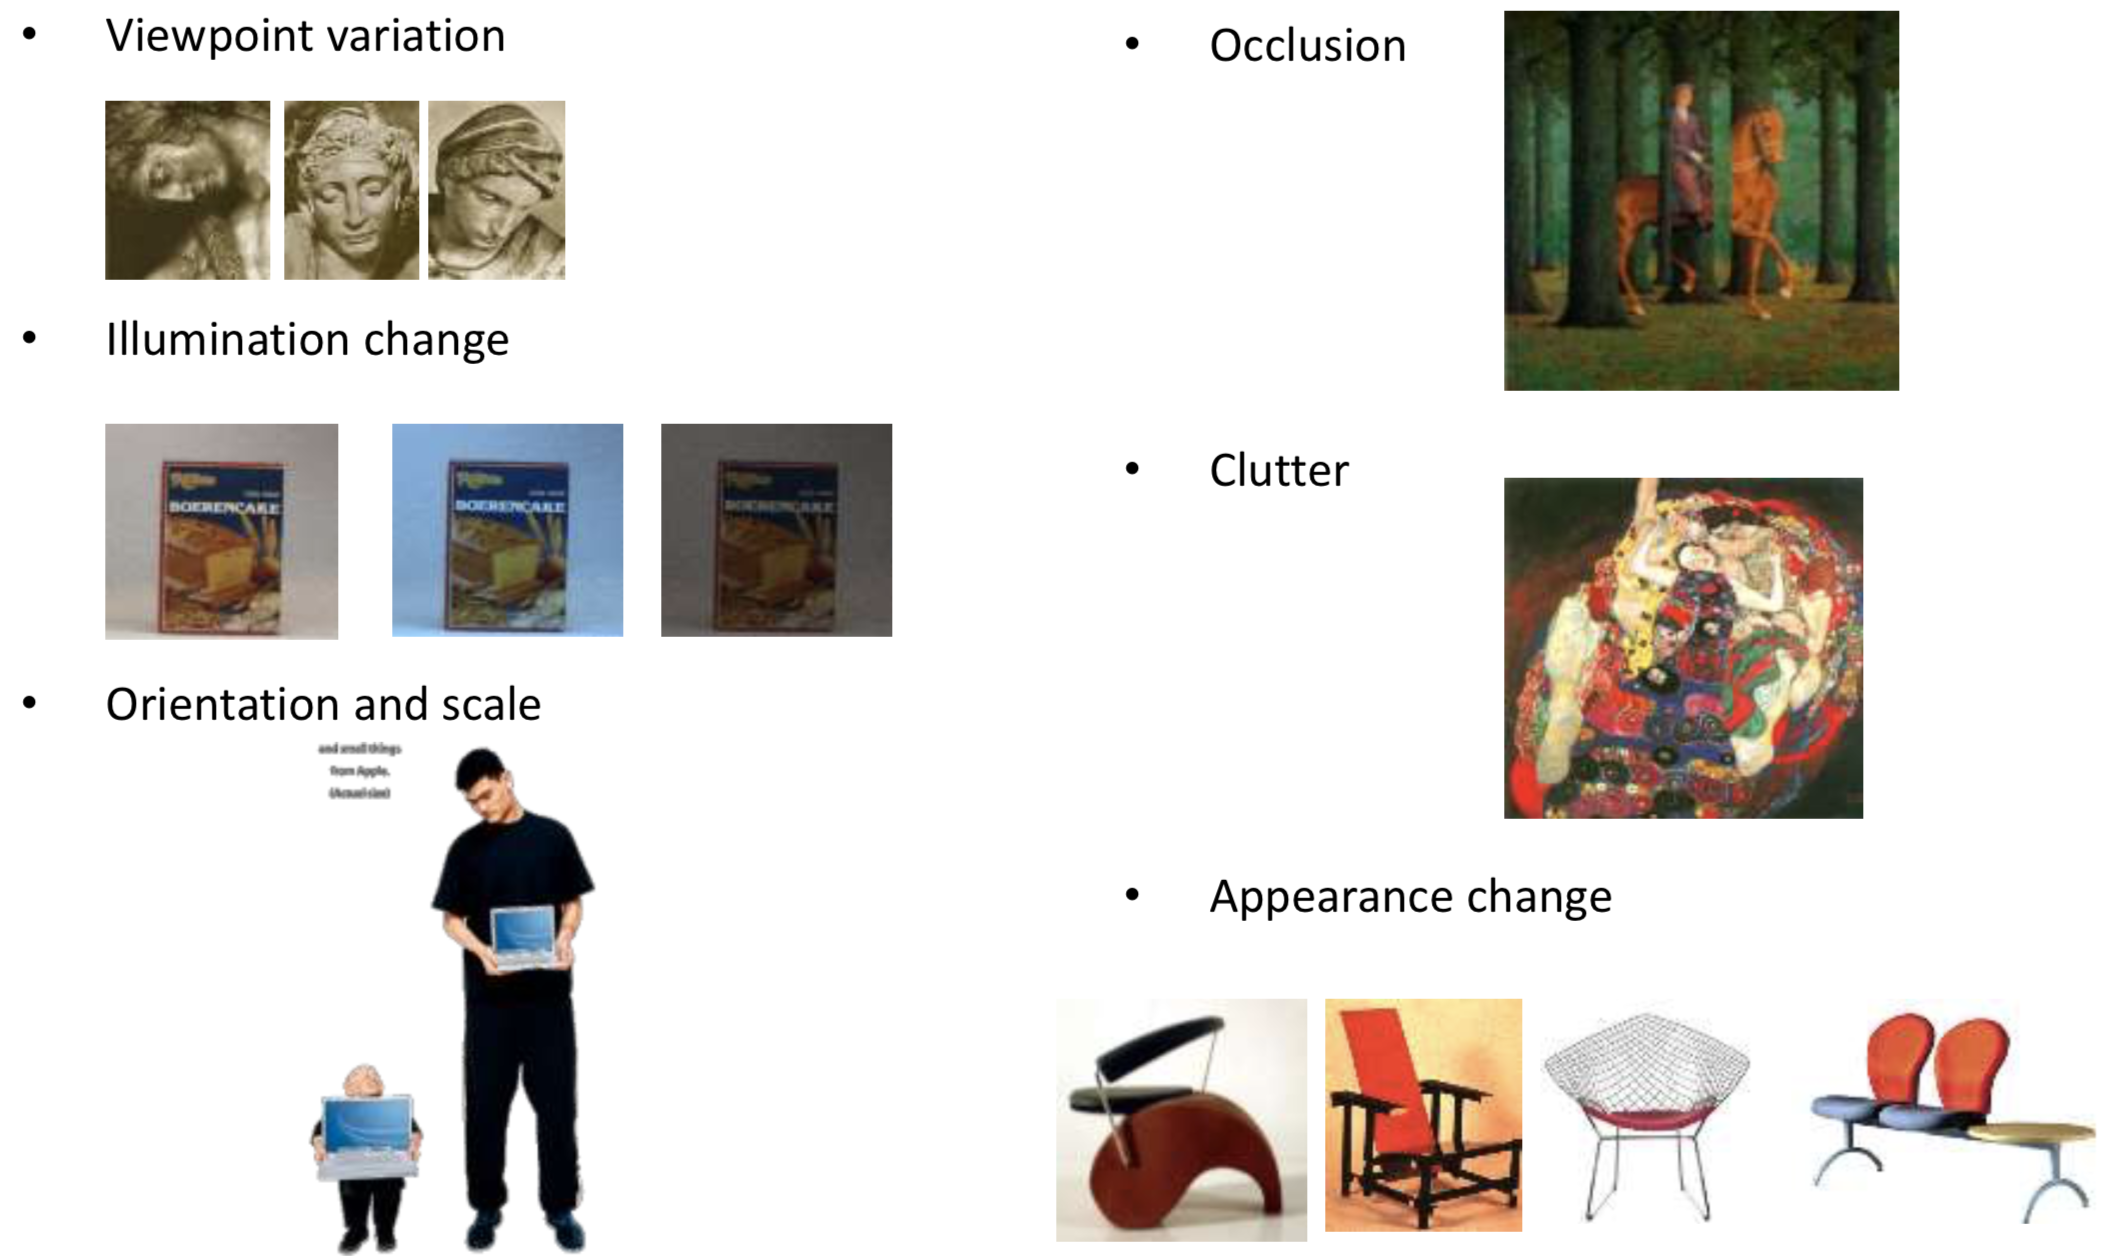
\includegraphics[width=0.5\textwidth]{figures/cv_image_formation_challenges_cv.png}
		\caption{Challenges in Computer Vision}
	\end{figure}
	\item The two main parts of how an image is formed are:
	\begin{itemize}
		\item \textit{Geometry} of the projection of a 3D environment to a 2D image. This defines which pixel belongs to which object (part/location). 
		\item \textit{Physics of light} which determines the brightness of a point in the image plane as a function of illumination and surface properties. Thus, the light source has a crucial influence on an object's appearance 
	\end{itemize}
\end{itemize}
\subsection{Projective Geometry and Camera models}
\begin{itemize}
	\item A camera can be abstracted by a pinhole model. Larger aperture/pinhole results in blurry images, smaller give sharp but noisy images (less energy of light is being passed) $\Rightarrow$ Change between both by using different lenses
	\item We represent an image by a projection plane. The intersection between the center of projection and the plane is determined by (note that $z$ is negative):
	$$(x,y,z)\to (-\frac{d}{z}\cdot x, -\frac{d}{z}\cdot y, -d)$$ 
	\begin{figure}[ht!]
		\centering
		\begin{subfigure}[b]{0.48\textwidth}
			\centering
			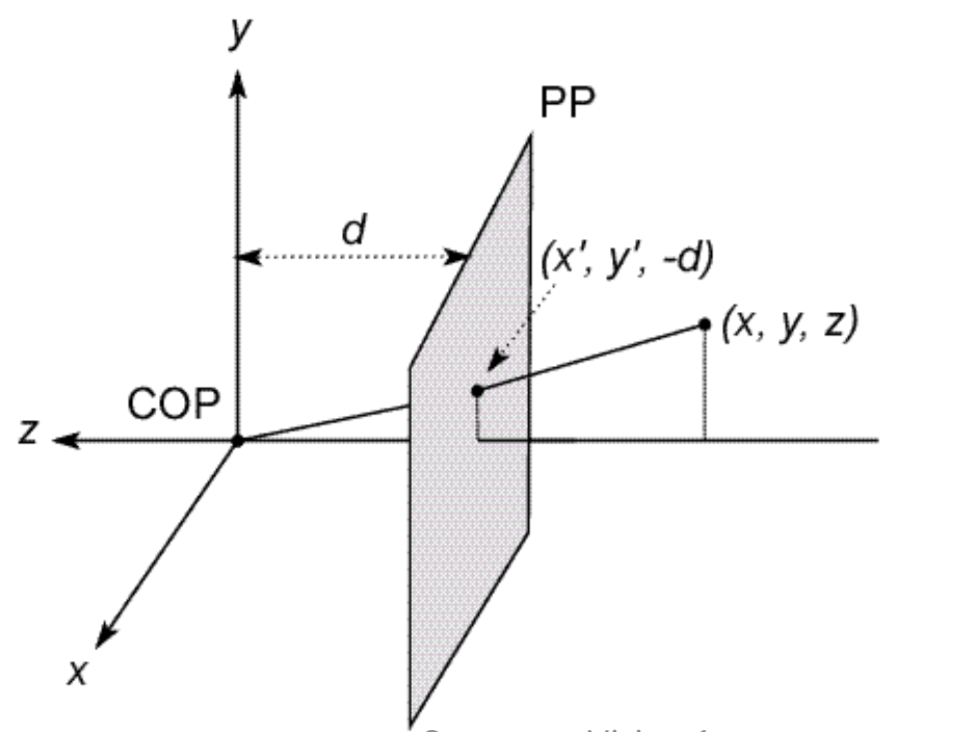
\includegraphics[width=0.4\textwidth]{figures/cv_image_formation_3D_model.png}
			\caption{Projection plane}
		\end{subfigure}
		\begin{subfigure}[b]{0.48\textwidth}
			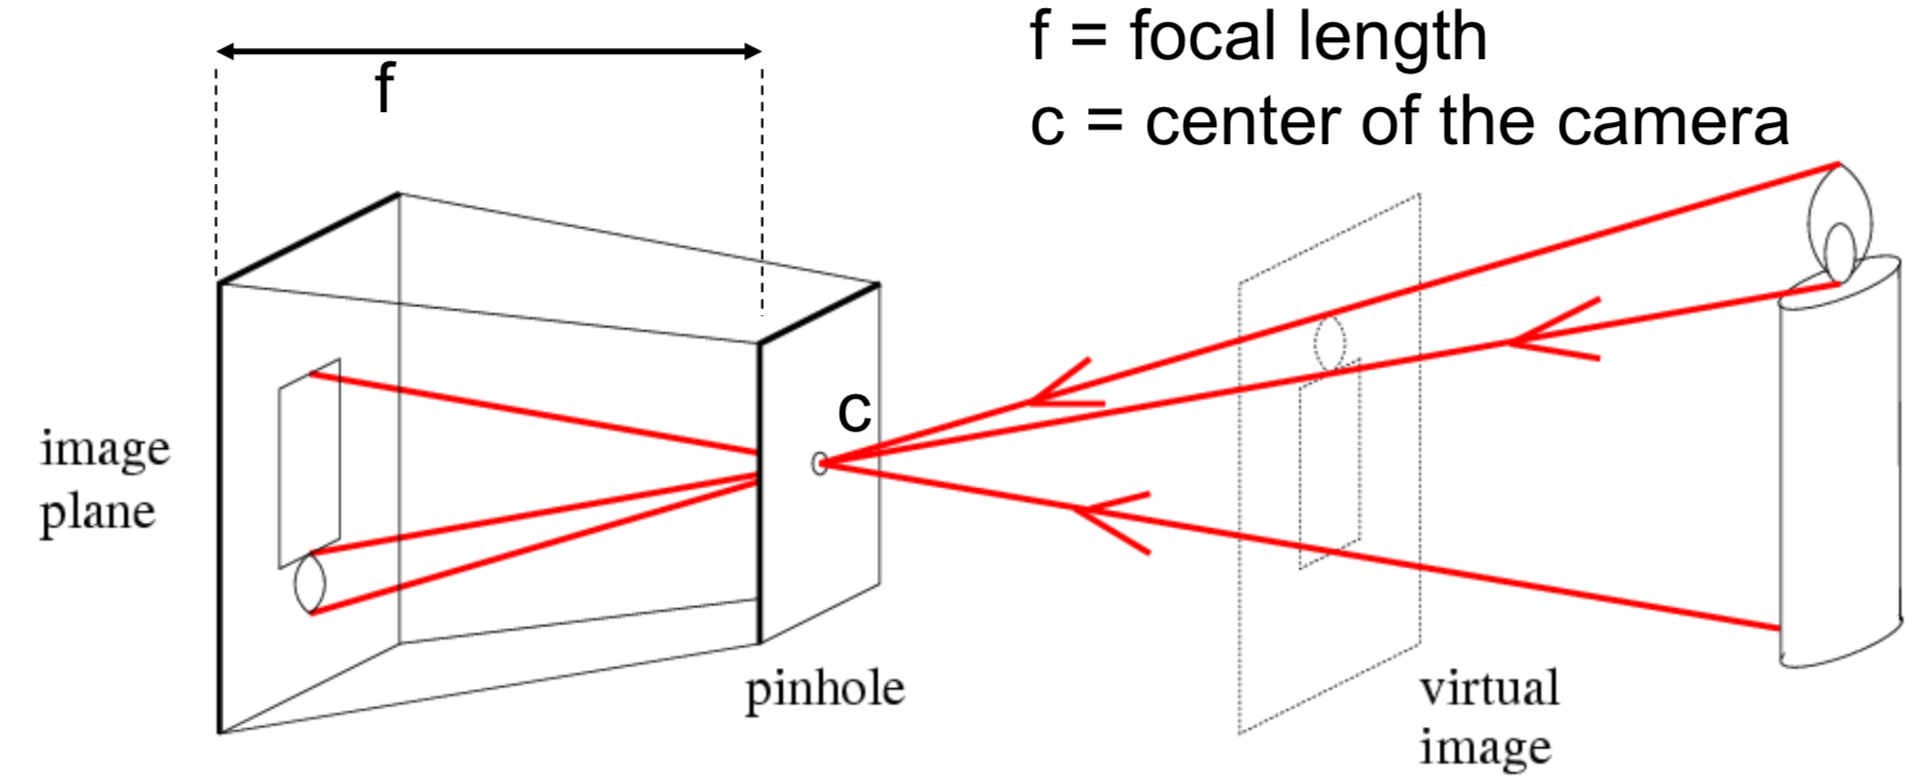
\includegraphics[width=0.8\textwidth]{figures/cv_image_formation_3D_model_2.png}
			\caption{Pinhole camera model}
		\end{subfigure}
		\caption{Abstract camera model in 3D coordinates}
	\end{figure}
	\item Model projection of 3D points to 2D image plane using homogeneous coordinates. The components we use for the projection are:
	\begin{itemize}
		\item \textit{Viewport projection}: Convert plane points to image coordinates (top left corner $(0,0)$, resolution scaling $s_x$, $s_y$)
		\item \textit{Perspective projection}: 3D points to image plane (homogeneous coordinates)
		\item \textit{View transformation}: rotation and translation matrix $\bm{R}$ and $\bm{T}$ for modeling the position and orientation of the camera. Can be seen as changing the coordinate system
		\item All together, we get the transformed points by:
		$$\left[\begin{array}{c}u\\v\\1\end{array}\right] = \underbrace{\left[\begin{array}{ccc}s_x & 0 & u_0\\0 & -s_y & v_0\\0 & 0 & 1\end{array}\right]}_{\text{Viewport}} \cdot \underbrace{\left[\begin{array}{cccc}1 & 0 & 0 & 0\\0 & 1 & 0 & 0\\0 & 0 & -1/d & 0\end{array}\right]}_{\text{Perspective}} \cdot \underbrace{\left[\begin{array}{cc}\bm{R} & \bm{T} \\\bm{0}^T_3 &  1\end{array}\right]}_{\text{View}} \cdot \left[\begin{array}{c}x\\y\\z\\1\end{array}\right]$$
	\end{itemize}
	\item Viewport and perspective projection depend on the camera (size and position of image plain) so that those are called \textit{intrinsic} camera parameter. In contrast, the view transformation is determined by \textit{extrinsic} camera parameters as it defines the camera position in the (original) coordinate system
\end{itemize}
\subsection{Light and Color models}
\label{sec:color_models}
\begin{itemize}
	\item The appearance color of an object is influenced by three components
	\begin{itemize}
		\item \textit{Light source}: spectral power distribution of light $e(\lambda)$ 
		\item \textit{Object}: the reflection distribution of an object $p(\lambda)$ (how good certain wavelengths are reflected)
		\item \textit{Sensor}: Detection by the sensor of the distribution $e(\lambda) p(\lambda)$
	\end{itemize}
	\item The goal is to be invariant to light source $e(\lambda)$ and sensor perspective
	\item Two very simple approaches to make an image independent of light source
	\begin{itemize}
		\item \textbf{Gray-world} assumption: the world is in average gray. So, we rescale every channel independently by $128/$mean of channel. Problematic if image is biased towards not being grey (high single channel, etc.)
		\item \textbf{Scale-by-max}/\textbf{White-patch} assumption: there is always at least one white pixel in an image. Hence, the channels are rescaled by $255$/max of channel. Fails if there is actually no white pixel in the image (results in wrong maximum), or if white pixel is in the shadow $\Rightarrow$ assumes whole image being shaded.
		\item All models underly/use the von Kries model where we convert an unknown light source $u$ to a canonical $c$ (i.e. day light) by simple channel scaling:
		$$\left(\begin{array}{c}R^c\\G^c\\B^c\end{array}\right) = \left(\begin{array}{ccc}
		\alpha & 0 & 0 \\
		0 & \beta & 0\\
		0 & 0 & \gamma
		\end{array}\right) \cdot \left(\begin{array}{c}R^u\\G^u\\B^u\end{array}\right)$$
		Note that to simplify the calculation of $\alpha$, $\beta$ and $\gamma$, and assume that the channels $R$, $G$ and $B$ are independent (thus only diagonal matrix), we approximate the integral as single wavelength for narrow-band filters.
	\end{itemize}
	\item As computer can't handle continuous distributions, the following integrals are approximate by for example the RGB model:
	$$R = \int_\lambda e(\lambda) p(\lambda) f_R(\lambda) d\lambda, \hspace{2mm}G = \int_\lambda e(\lambda) p(\lambda) f_G(\lambda) d\lambda, \hspace{2mm}B = \int_\lambda e(\lambda) p(\lambda) f_B(\lambda) d\lambda$$
	Every spectral color (see below diagram in Figure~\ref{fig:rgb_color_wavelength_distribution_RGB}) can be represented by an linear combination of RGB values.
	Note that human ganglion cells have similar functions, but are the most sensitive to green.
	\begin{figure}[ht!]
		\centering
		\begin{subfigure}[b]{0.4\textwidth}
			\centering
			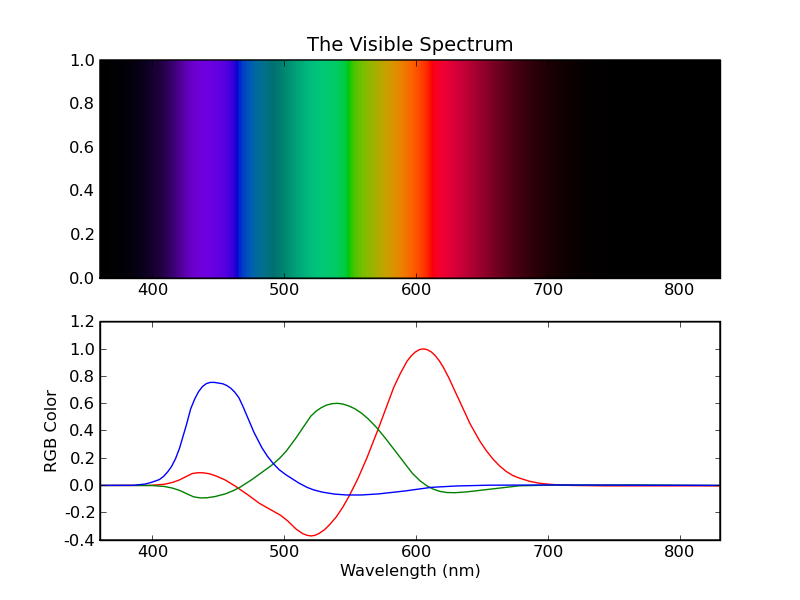
\includegraphics[width=0.75\textwidth]{figures/cv_image_formation_color_RGB_model.png}
			\caption{RGB model}
			\label{fig:rgb_color_wavelength_distribution_RGB}
		\end{subfigure}
		\begin{subfigure}[b]{0.24\textwidth}
			\centering
			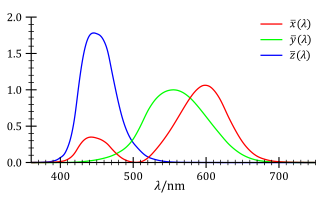
\includegraphics[width=\textwidth]{figures/cv_image_formation_color_XYZ_model.png}
			\caption{XYZ model}
			\label{fig:rgb_color_wavelength_distribution_XYZ}
		\end{subfigure}
		\hspace{5mm}
		\begin{subfigure}[b]{0.28\textwidth}
			\centering
			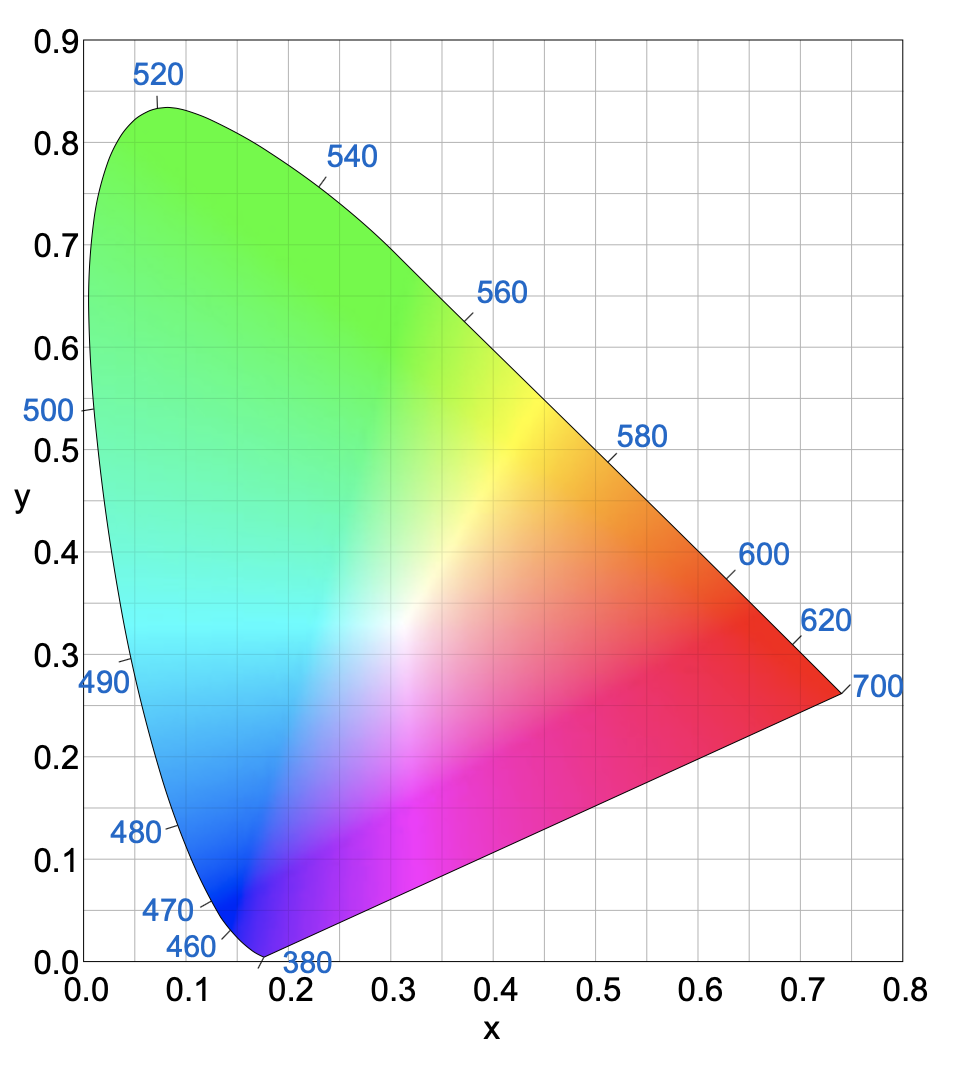
\includegraphics[width=0.8\textwidth]{figures/cv_image_formation_color_XYZ_diagram_2.png}
			\caption{XYZ diagram}
			\label{fig:rgb_color_wavelength_distribution_XYZ_diagram}
		\end{subfigure}
		\caption{Color matching functions $f_R$, $f_G$ and $f_B$ for the standard (a) RGB / (b) XYZ model. The colors represented by the XYZ system are shown in (c). Note that the line of purples contains colors that cannot be created by a monochromatic light source and needs a combination of fully saturated red and violet (max and min of spectrum).}
		\label{fig:rgb_color_wavelength_distribution}
	\end{figure}
	\item The intensity of the RGB color space is calculated by the sum of the channels: $I=R+G+B$
	\item Another color space is the XYZ system. The color matching functions $\overline{x}(\lambda), \overline{y}(\lambda), \overline{z}(\lambda)$ are similar but not the same as RGB (see Figure~\ref{fig:rgb_color_wavelength_distribution_XYZ}). The values are calculated by:
	$$X = \int_\lambda e(\lambda) p(\lambda) \overline{x}(\lambda) d\lambda, \hspace{2mm}Y = \int_\lambda e(\lambda) p(\lambda) \overline{y}(\lambda) d\lambda, \hspace{2mm}Z = \int_\lambda e(\lambda) p(\lambda) \overline{z}(\lambda) d\lambda$$
	\item However, we can split these measurements into a brightness/luminance and chromaticity/color component specified by $x$ and $y$. The luminance is given by $Y$ ($XYZ$ was designed for that), and the chromaticity is determined as ($Z$ is implicitly given by $1-x-y$):
	$$x=\frac{X}{X+Y+Z},\hspace{2mm}y=\frac{Y}{X+Y+Z}$$
	\item The created colors can be visualized in an $xy$-diagram (see Figure~\ref{fig:rgb_color_wavelength_distribution_XYZ_diagram}). 
	\item Given a reference light source $e$, we can determine the dominant wavelength (\textit{hue}) of a point $p$ by a line from $e$ through $p$ towards the boundary. The \textit{saturation} is given by the ratio of line length between $e$ and $p$ and $e$ to dominant wavelength boundary. Combining these with the luminance $Y$, a point $p$ can be converted into the HSI color space (see Figure~\ref{fig:rgb_color_HSV_color_cone}).
	\item HSV can be seen as applying non-linear functions on the wavelength distribution (see Figure~\ref{fig:rgb_color_HSV_wavelength_dist}). Hue is defined as the dominant wavelength, saturation as the purity of the color (probably relation between max energy and mean), and the brightness/luminance (given by average)
	\begin{figure}[ht!]
		\centering
		\begin{subfigure}[b]{0.4\textwidth}
			\centering
			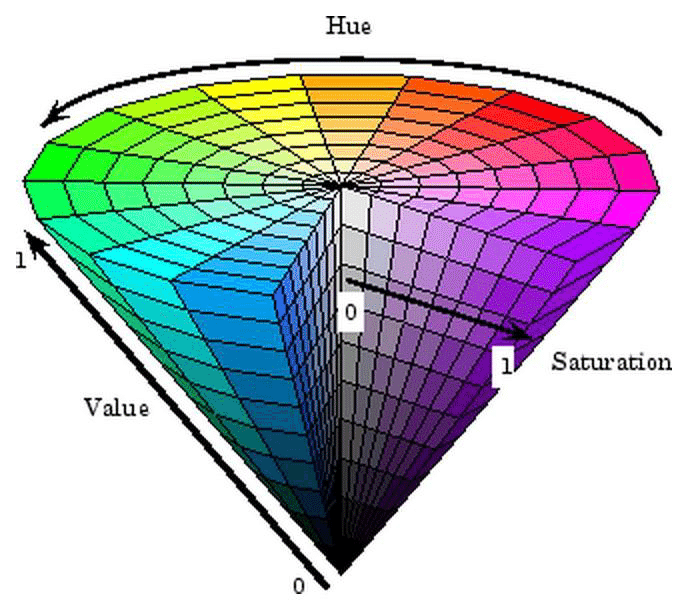
\includegraphics[width=0.5\textwidth]{figures/cv_image_formation_color_HSV.png}
			\caption{HSV color cone}
			\label{fig:rgb_color_HSV_color_cone}
		\end{subfigure}
		\begin{subfigure}[b]{0.4\textwidth}
			\centering
			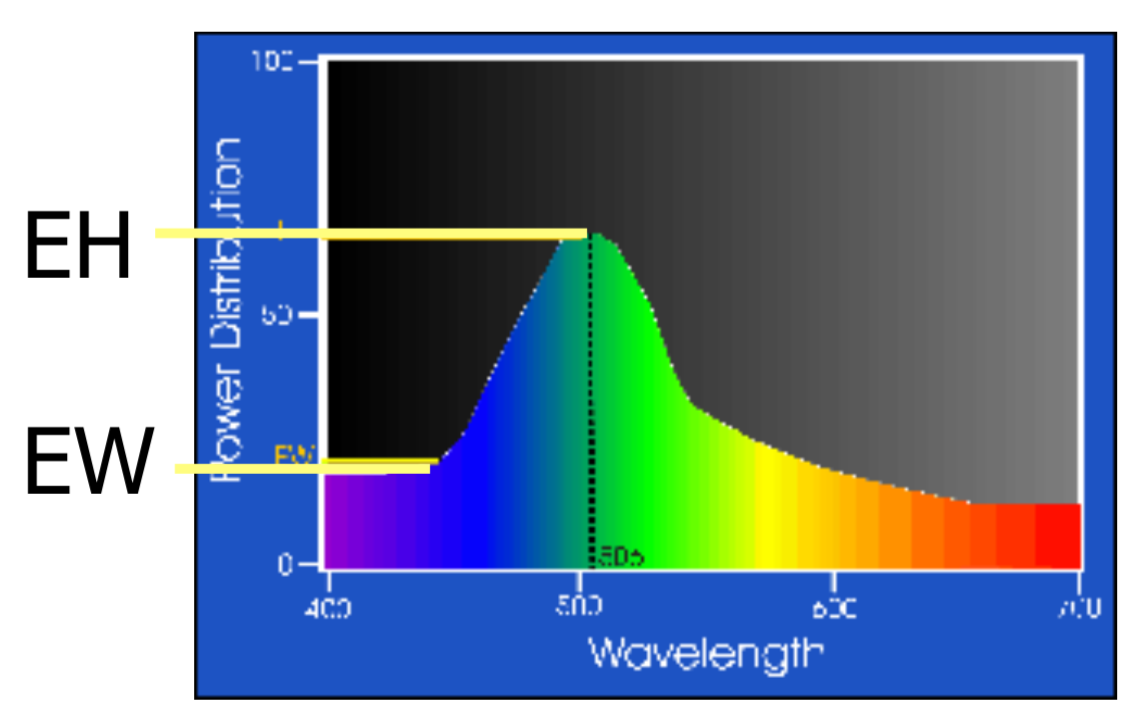
\includegraphics[width=0.6\textwidth]{figures/cv_image_formation_color_HSV_wavelength_dist.png}
			\caption{HSV wavelength distribution}
			\label{fig:rgb_color_HSV_wavelength_dist}
		\end{subfigure}
		\caption{HSV color space. }
	\end{figure}
	\item The $xy$-diagram in Figure~\ref{fig:rgb_color_wavelength_distribution_XYZ_diagram} visualizes the gamut that is visible for an average person/human vision. Different color spaces/devices capture colors by defining three points and linearly interpolate between those. However, it can be seen that there is no such gamut that can include the whole human vision gamut.
\end{itemize}
\subsection{Reflection models}
\begin{itemize}
	\item When a light source shines on an object, it might be differently perceived from different sensors/cameras although they have the same properties $\Rightarrow$ object appearance by reflectance
	\item The reflectance properties of an object/point can be specified by a \textit{BRDF}: Bi-directional reflectance distribution function $f(\theta_i, \phi_i; \theta_r, \phi_r)$ ($\theta_i$ and $\phi_i$ define the angles between input light and surface normal in $x$-$z$/$x$-$y$ direction respectively, $\theta_r$ and $\phi_r$ for the outgoing direction).
	\item A BRDF can be build up by different components, as visualized in Figure~\ref{fig:reflection_models_brdf_reflection_components}. The main parts can be distinguished into \textit{body reflection} (also referred to as mate appearance), and \textit{surface reflection} (responsible for the glossy appearance)
	\begin{figure}[ht!]
		\centering
		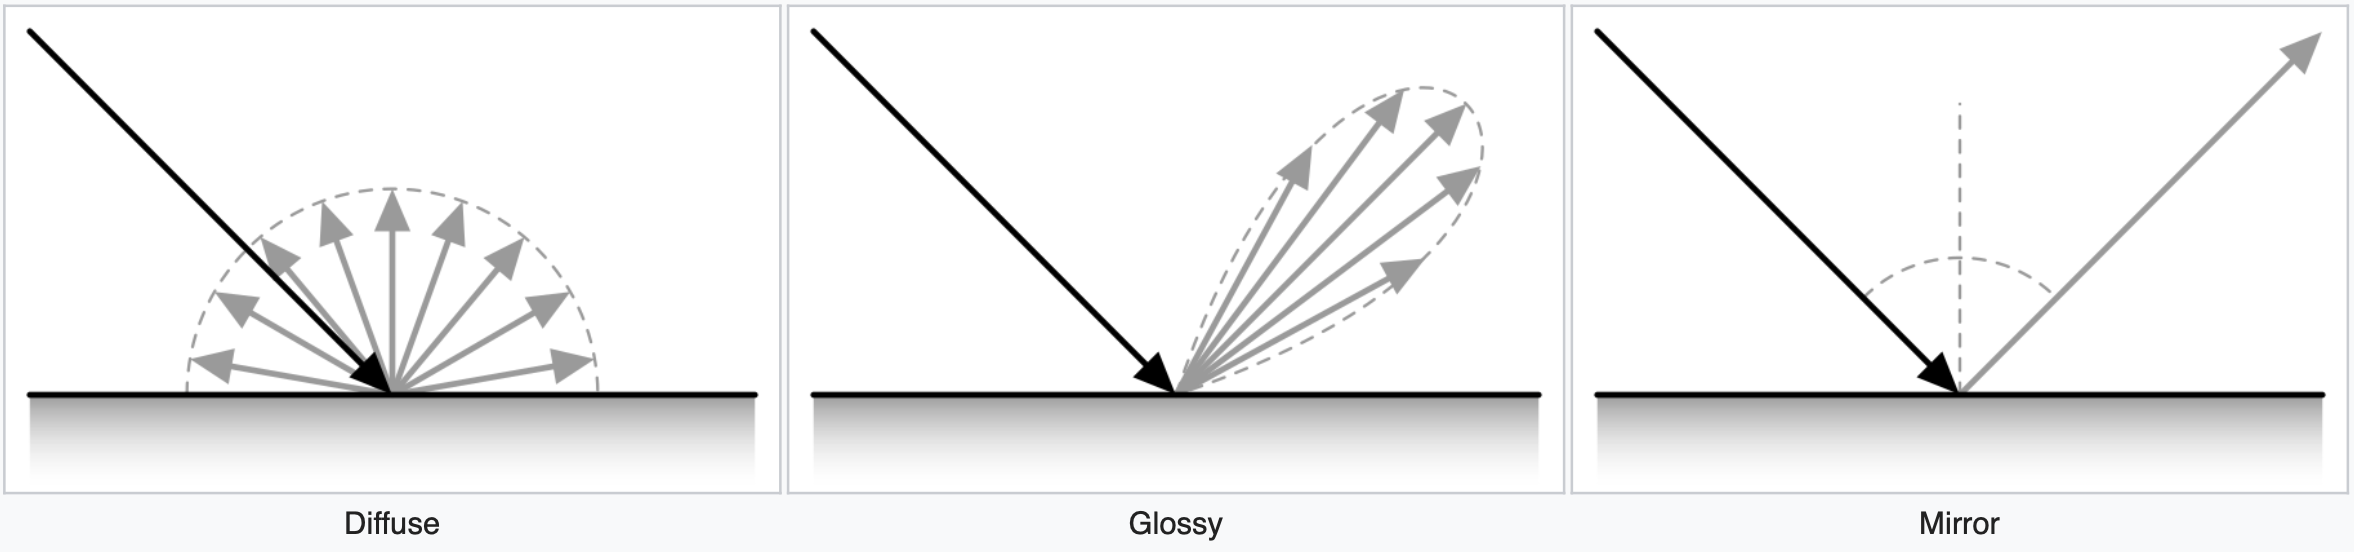
\includegraphics[width=0.8\textwidth]{figures/cv_image_formation_reflectance_properties.png}
		\caption{Different components of reflectance. Black arrow visualizes the input ray, and greyish/shaded arrows the output rays. Length of the output rays indicate their energy. }
		\label{fig:reflection_models_brdf_reflection_components}
	\end{figure}
	\item There are different models that approximate/assume/deal with certain forms of BRDFs
\end{itemize}
\subsubsection{Lambertian model}
\begin{itemize}
	\item The lambertian reflectance model assumes a BRDF that constant: $f(\theta_i, \phi_i; \theta_r, \phi_r) = \frac{\rho_d}{\pi}$ where $\rho_d$ is defined by the albedo of the object, and division of $\pi$ as energy is equally distributed over hemisphere
	\item The surface reflection/output radiance can be calculated by $L=\frac{\rho_d}{\pi}I\cos \theta_i=\frac{\rho_d}{\pi}I\cdot (\vec{n}\cdot \vec{s})$ where $I$ is light source intensity, $\vec{n}$ the surface normal and $\vec{s}$ the input ray direction.
	\item Note that the factor $(\vec{n}\cdot \vec{s})$ defines the ratio of energy/photons that interact with that point/surface
	\item By assuming a Lambertian world, we can decompose an image into a shading part (surface normals) and the albedo (reflectance) of an object.
\end{itemize}
\subsubsection{Phong model}
\begin{itemize}
	\item The Phong model extends the Lambertian model by taking glossy reflectance into account (note that mirror is mostly approximated by glossy as mirror only looks at a single output angle which is rarely met). See Figure~\ref{fig:reflection_models_phong} for the components of the Phong model
	\begin{figure}[ht!]
		\centering
		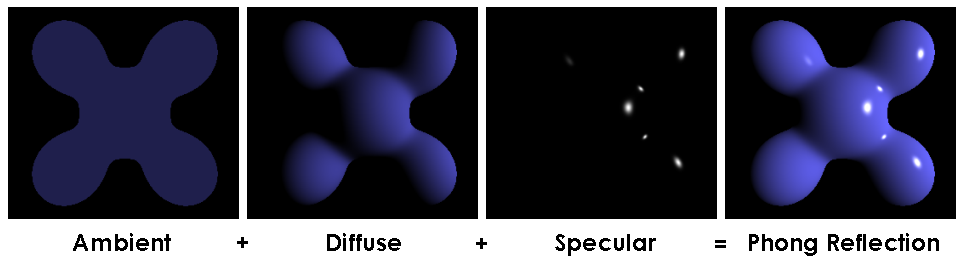
\includegraphics[width=0.7\textwidth]{figures/cv_image_formation_phong_model.png}
		\caption{The Phong model combines diffuse and glossy reflectance. Note that ambient gives the object a certain base brightness for approximating reflectance among objects/walls/...}
		\label{fig:reflection_models_phong}
	\end{figure}
	\item The reflection component of the specularity is calculated by $L_s=I\cdot \rho_s \left(\cos \phi\right)^{n_{shiny}}=I\cdot \rho_s \left(\vec{r}\cdot \vec{v}\right)^{n_{shiny}}$ where $r$ is the output ray/mirror direction (calculated by $\vec{r}=2\cdot \vec{n} \cdot (\cos \theta) - \vec{s}$), and $v$ the view direction of the sensor. 
	\item Large values for $n_{shiny}$ lead to narrow, small dot reflections (close to mirror) while small $n_{shiny}$ give broad, big surface reflectance. Note that the intensity is capped at a highest value (e.g. 1 or 255), so that multiple points can have the maximum intensity although they have a slightly different angle
	\item Also, Figure~\ref{fig:reflection_models_phong} shows that the body reflection (diffuse and ambient) contain the object color while the specularity depends on the light source (highlights color from light source)
\end{itemize}
\subsubsection{Dichromatic reflection models}
\begin{itemize}
	\item The previously discussed models only consider the light source intensity for the reflection. However, we can integrate the reflection in our color models:
	$$\text{body}_C = m_b (\vec{n}, \vec{s})  \int_\lambda e(\lambda) p(\lambda) f_C(\lambda) d\lambda$$
	$$\text{surface}_C = m_s (\vec{n}, \vec{s}, \vec{v})  \int_\lambda e(\lambda) c(\lambda) f_C(\lambda) d\lambda$$
	where $C$ is a specific channel (for example $R$, $G$ or $B$), $\vec{n}$ is the surface normal, $\vec{s}$ the input ray direction and $\vec{v}$ the viewpoint. 
	\item The function $m_b$ models the diffuse body reflection (i.e. $m_b(\vec{n}, \vec{s})=\cos \theta = \vec{n}\cdot \vec{s}$ as for Lambertian) whereas $m_s$ represents the glossy surface reflection (i.e. Phong model). 
	\item The diffuse reflectance depends on the albedo of the object $p(\lambda)$ whereas $c(\lambda)$ determines the specularity of the object for certain wavelengths.
	\item The perceived color of an object is the sum of the body and the surface
	\item Our goal is to map an input image into a space which is independent of the scene (i.e. independent of $m_b$, $m_s$, ...). Different color models can help:
	\begin{itemize}
		\item \textbf{rgb}: Assuming a white light source, normalize RGB values by the intensity (i.e. $r=\frac{R}{R+G+B}$). This leads to photometric invariance for pure matte objects ($m_b$ cancels out as it is the same for all channels when assuming $m_s=0$). Note that this approach fails if an object has no color (i.e. all gray tones are mapped to the same value).
		\item \textbf{c1c2c3}: color space is obtained from RGB manipulation and is invariant to shadowing effects of light interaction particularly for matte objects. It has similar properties as rgb, but is determined by $c_1(R,G,B) = \arctan\frac{R}{\max\left\{G,B\right\}}$
		\item \textbf{HSV} can be invariant to specularity if we assume a white light source and thus white specularity. The dominant wavelength, i.e. the hue, stays the same for those points. However, note that this model is instable for gray and especially white points that commonly occur at maximum specularity, as the hue is undefined.
		\item \textbf{l1l2l3}: Similar behavior as HSV, but calculates the values by $l_1(R,G,B) = \frac{(R-G)^2}{(R-G)^2 + (R-B)^2 + (G-B)^2}$
	\end{itemize}
	\item Figure~\ref{fig:cv_image_formation_invariance_color_spaces} summarizes some invariance properties of common color spaces
	\begin{figure}[ht!]
		\centering
		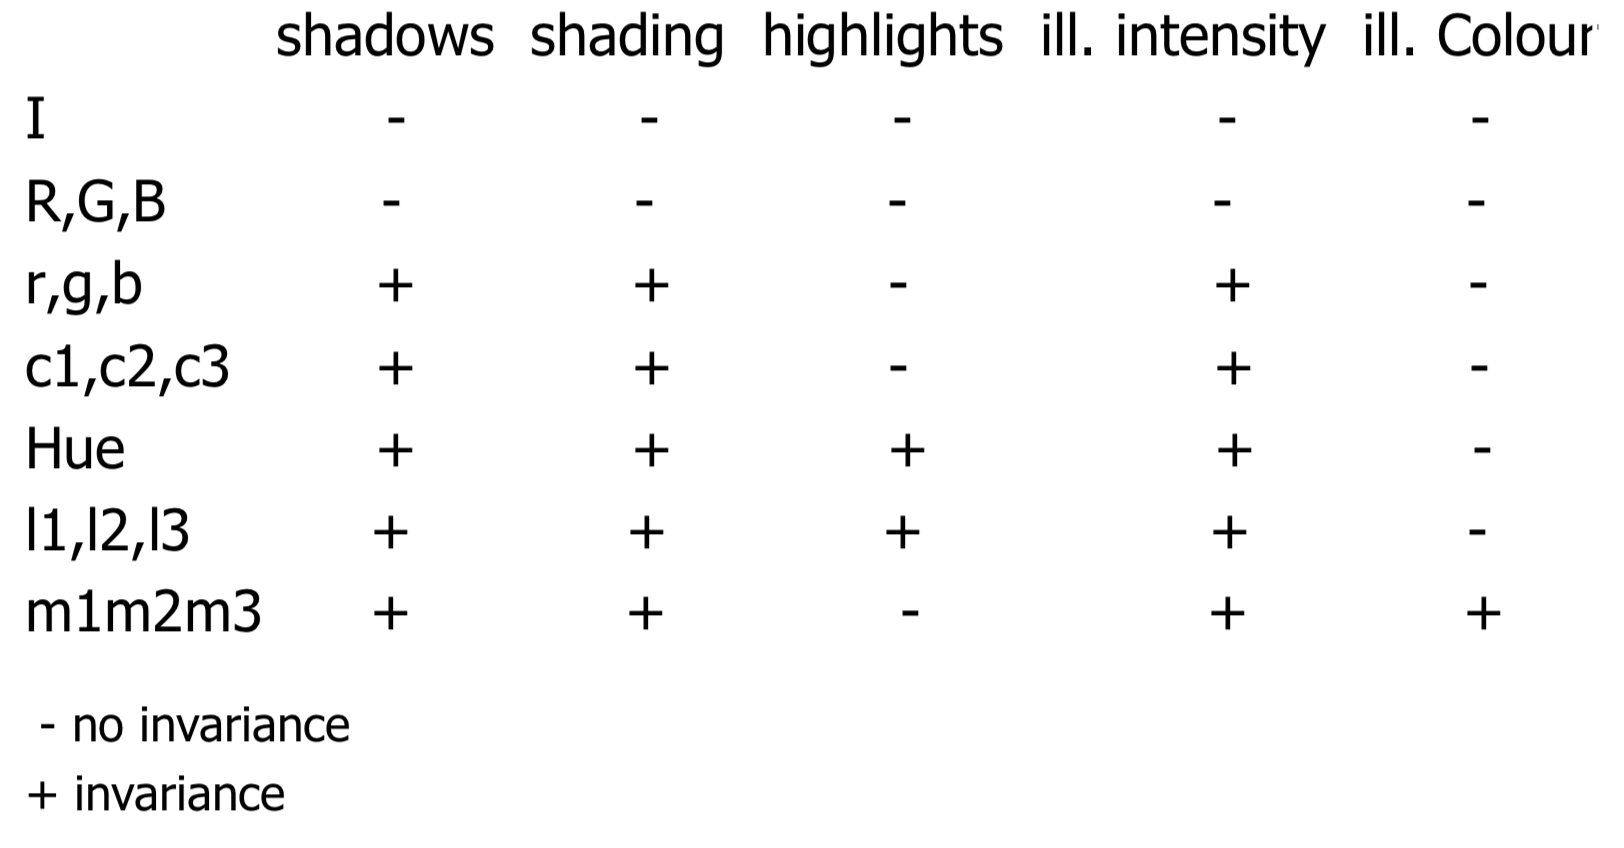
\includegraphics[width=0.5\textwidth]{figures/cv_image_formation_invariance_color_spaces.png}
		\caption{Overview of invariance in color spaces.}
		\label{fig:cv_image_formation_invariance_color_spaces}
	\end{figure}
	\item Different color spaces have different instabilities. Normalized colors get unstable around black pixels ($R=1, G=0, B=0$ is considered as pure red in rgb although in RGB it is black) whereas Hue is instable for low saturation (any hue gives same color)
	\item Another method to be invariant to shadows is filtering the image for smooth image intensity transitions as color transitions are harsh compared to that. The new image is recovered by summing up over gradients. Note that this method fails for sharp shadows and/or smooth color transitions
\end{itemize}
\section{Image processing}
\begin{itemize}
	\item Apply various algorithms on image to analyze/improve the data
	\item The simplest kind of image transformation are those independent to the spatial position (thus also called point processing) where the new image is calculated by $g=a\cdot t(f)+ b$. Examples: gamma correction ($\log x$ to boost small, black values more than high ones), histogram equalization
\end{itemize}
\subsection{Neighborhood processing}
\begin{itemize}
	\item The most common way to process an image is by applying filters on it. A filter is a linear weighted sum of local input values. 
	\item A convolution of image $I$ and a linear filter $h$ is calculated by $$I_{out} = I \ast h, \hspace{1mm} I_{out}(i,j) = \sum\limits_{k,l} I(i-k, j-l) \cdot h(k,l)$$
	\item Depending on the size of the filter, we might not be able to apply the filter on the pixels at the border. Thus, we extend the image to have the same output shape. Common padding methods are zero/black, mirror/copy edge or wrap around.
	\item There are a lot of different filters that can be applied on an image. Filters can for example also be used for translation if wanted/needed. 1D example: $\left[\begin{array}{ccc}
	0 & 0 & 1
	\end{array}\right]$
	\item In general, we distinguish between \textit{low}-pass filters (smoothing) and \textit{high}-pass filters (edge detection, sharpening). The frequency is thereby the change of pixel values, and the passed wavelengths describe to what the filters react the most. Note that there are also \textit{band}-pass filters (low-pass filter convolved with high-pass filter)
	\item For example, unicolor images stay mostly unchanged when they are processed by an low-pass filter. In contrast, applying a high-pass filter on such images leads to very low activations.
\end{itemize}
\subsubsection{Smoothing filters}
\begin{itemize}
	\item \textit{Box filter}: replace every pixel by the average of its neighborhood. 
	$$h = \frac{1}{9}\left[\begin{array}{ccc}
	1 & 1 & 1\\
	1 & 1 & 1\\
	1 & 1 & 1\\
	\end{array}\right]$$
	Convolving a box filter with itself results in a filter in a shape of a Gaussian
	\item \textit{Gaussian filter}: weight contributions of neighboring pixels by distance: $G_\sigma = \frac{1}{2\pi \sigma^2} e^{-\frac{(x^2 +y^2)}{2\sigma^2 }}$. A $3\times 3$ Gaussian with $\sigma=0.5$ has the following values:
	$$h= \left[\begin{array}{ccc}
	0.011 & 0.084 & 0.011\\
	0.084 & 0.619 & 0.084\\
	0.011 & 0.084 & 0.011\\
	\end{array}\right]$$
	Note that convolving a Gaussian with another Gaussian is again a Gaussian. Thus, we can separate a 2D Gaussian into two 1D filters which are sequentially applied on the image $\Rightarrow$ reduce computational effort from $n^2$ to $2n$.
	\item \textit{Sharpening filter}: reverses the process of smoothing by accentuates differences with local average
	$$h = \left[\begin{array}{ccc}
	0 & 0 & 0\\
	0 & 2 & 0\\
	0 & 0 & 0\
	\end{array}\right]-\frac{1}{9}\left[\begin{array}{ccc}
	1 & 1 & 1\\
	1 & 1 & 1\\
	1 & 1 & 1\\
	\end{array}\right]$$
	\item \textit{Median filter}: A non-linear filter that selects the median value in the kernel window. The advantage of this filter is that its robust against outliers (good for filtering out salt-and-pepper noise)
\end{itemize}
\subsubsection{Edge detection filters}
\begin{itemize}
	\item \textit{Simple gradient filter}: The simplest gradient/edge detector is in 1D: $h = \left[\begin{array}{cc}-1 & 1\end{array}\right]$ 
	\item \textit{Sobel filter}: a derivative filter that also takes nearby pixels into account for better approximation. $h_x$ detects vertical edges (gradients over $x$-direction) and $h_y$ detects horizontal edges.
	$$h_x = \left[\begin{array}{ccc}
	1 & 0 & -1\\
	2 & 0 & -2\\
	1 & 0 & -1\\
	\end{array}\right] \text{\hspace{5mm}and\hspace{5mm}}h_y = \left[\begin{array}{ccc}
	1 & 2 & 1\\
	0 & 0 & 0\\
	-1 & -2 & -1\\\end{array}\right] $$ 
	\item \textit{Derivative of a Gaussian}: the derivative of a Gaussian is highly suitable for edge detection as it represents a band-pass filter (Gaussian filter convolved with discrete gradient filter although derivative mostly calculated by continuous). Similar to sobel, but weights the pixels nearby a bit different. Note that we also have different filters for $x$ and $y$ direction.
	\item \textit{Laplacian of Gaussian}: Laplacian operator $\nabla^2 f = \frac{\partial^2 
	f}{\partial x^2} + \frac{\partial^2 f}{\partial y^2}$ applied on a Gaussian. Is invariant to the direction of the gradient (circular symmetric). The shape of the function is also often described as a Mexican hat (see Figure~\ref{fig:cv_image_processing_gaussian_filters}). Is highly responsive to blobs (blob detection) but is sensitive to the scale. To be invariant of the scale, we can apply multiple LoG filters with different values of $\sigma$ and stack the results together.
	\begin{figure}[ht!]
		\centering
		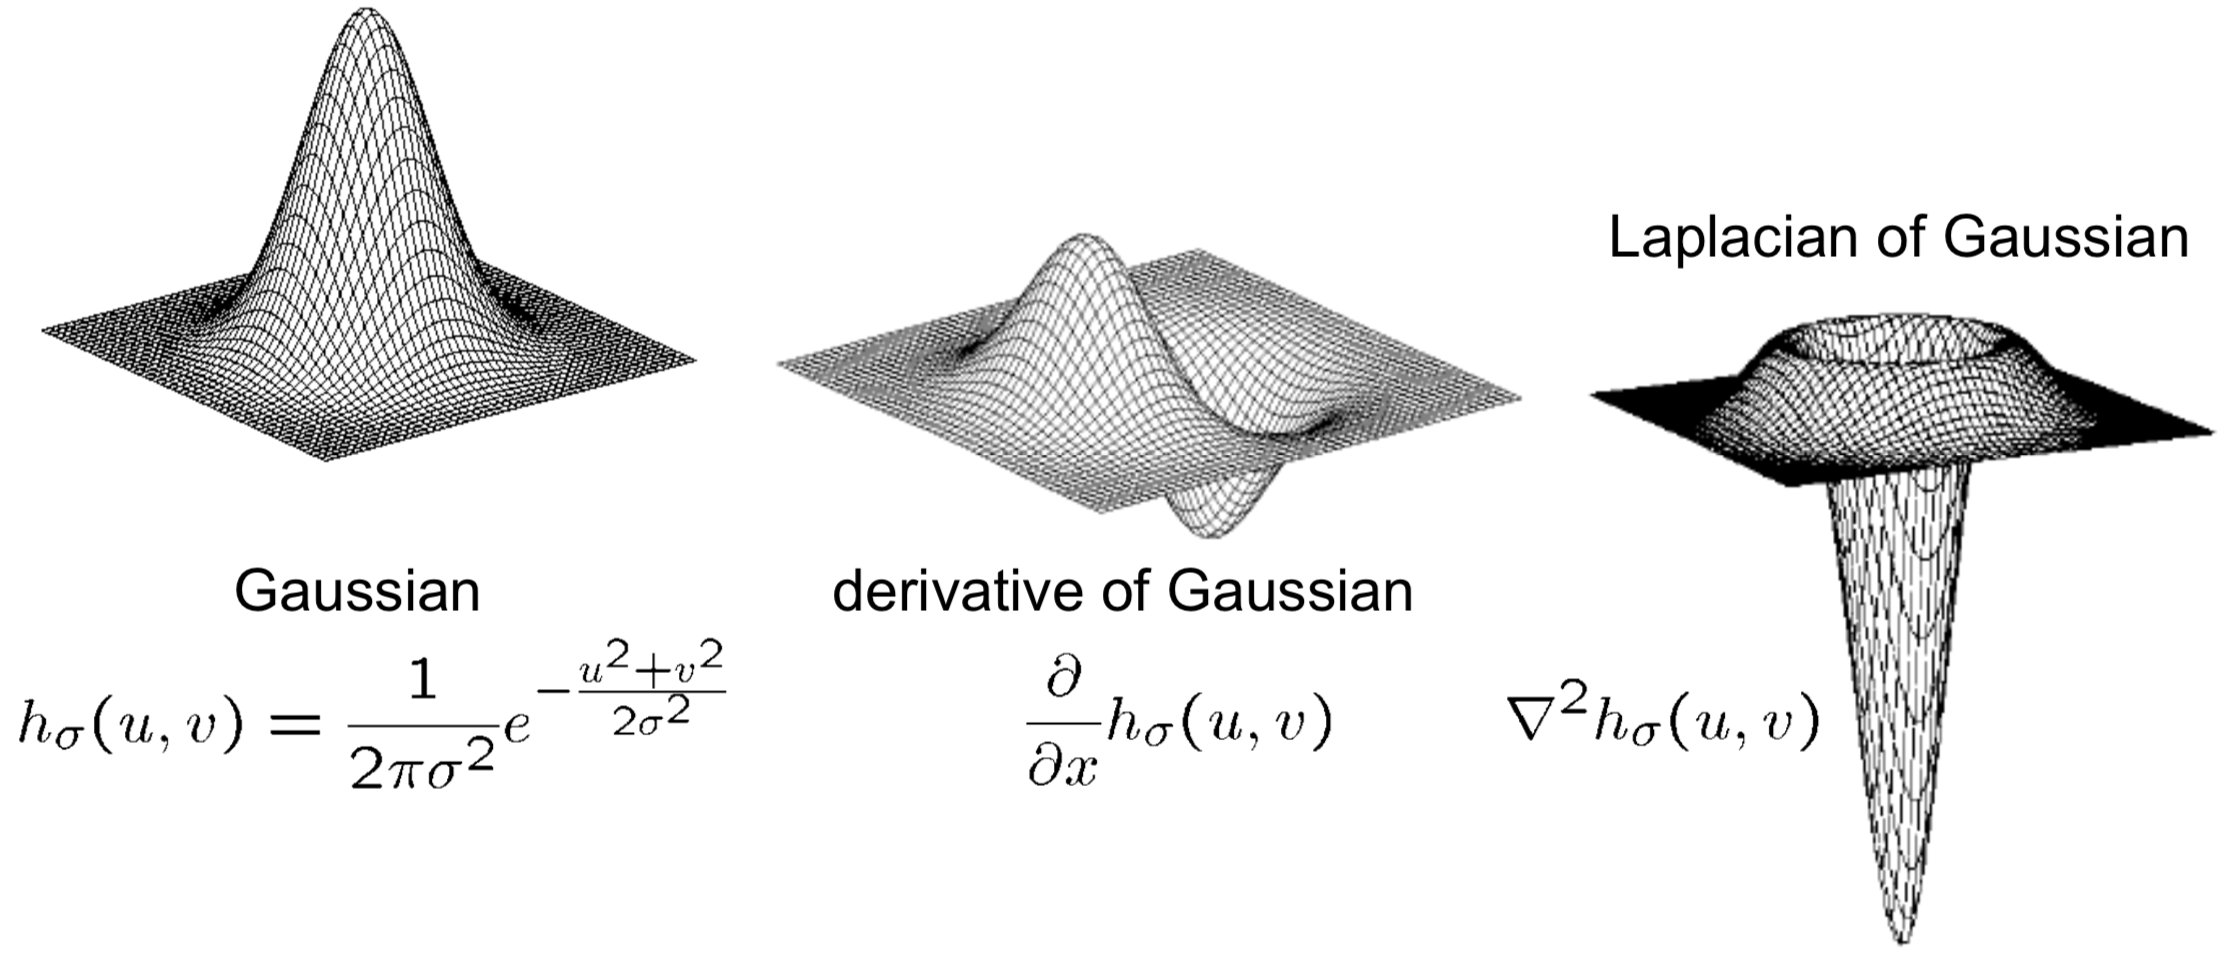
\includegraphics[width=0.6\textwidth]{figures/cv_image_processing_gaussian_filters.png}
		\caption{Visualization of different Gaussian filters.}
		\label{fig:cv_image_processing_gaussian_filters}
	\end{figure}
\end{itemize}
\subsection{Harris corner detector}
\begin{itemize}
	\item Detect interest points in an image to perform matching or similar tasks. Corners are suitable to serve as interest points as they have a unique 2D position compared to edges and points
	\item The initial idea is derived from performing autocorrelation on a small window of the image, and test which ones are unique/expressive. Now we are looking for small changes in $x$ and $y$ direction, how much the image changes. Based on that information, we can decide whether a pixel represents a corner or not.
	\item Steps in the Harris corner detector
	\begin{enumerate}
		\item Compute the derivatives $I_x$ and $I_y$ of the image
		\item Compute the products of the derivatives at every pixel: $I_x^2$, $I_y^2$, $I_{xy}=I_{x}\cdot I_{y}$ 
		\item Compute sums of products over the window size and align them in the Harris matrix:
		$$H = \left[\begin{array}{cc}
		\sum_W I_x^2 & \sum_W I_x \cdot I_y\\
		\sum_W I_x \cdot I_y & \sum_W I_y^2 \\
		\end{array}\right]$$
		Note that the sum represents the application of a box filter. It is equally possible to apply Gaussian filters etc. 
		\item Determine the response of the detector at each pixel:
		$$R = \det(H) - k\cdot \left(\text{trace}(H)\right)^2$$
		\item If $|R|$ is small, the region is probably flat. Otherwise, if $R<0$ (and greater a certain threshold) we have an edge, and $R>0$ indicates a corner.
		\item Perform non-maximum suppression if corner detector is calculated pixel-wise.
	\end{enumerate}
	\item Determining the \textit{cornerness} of a point is based on the eigenvalues of the matrix $H$: $R=\lambda_1 \lambda_2 - k\cdot (\lambda_1 + \lambda_2)^2$. The maximum eigenvalue is the gradient of the direction with the fastest change, and the minimum eigenvalue the gradient of the direction with the smallest change. Note that this models an ellipse for the gradients (see Figure~\ref{fig:cv_image_processing_harris_ellipse})
	\begin{figure}[ht!]
		\centering
		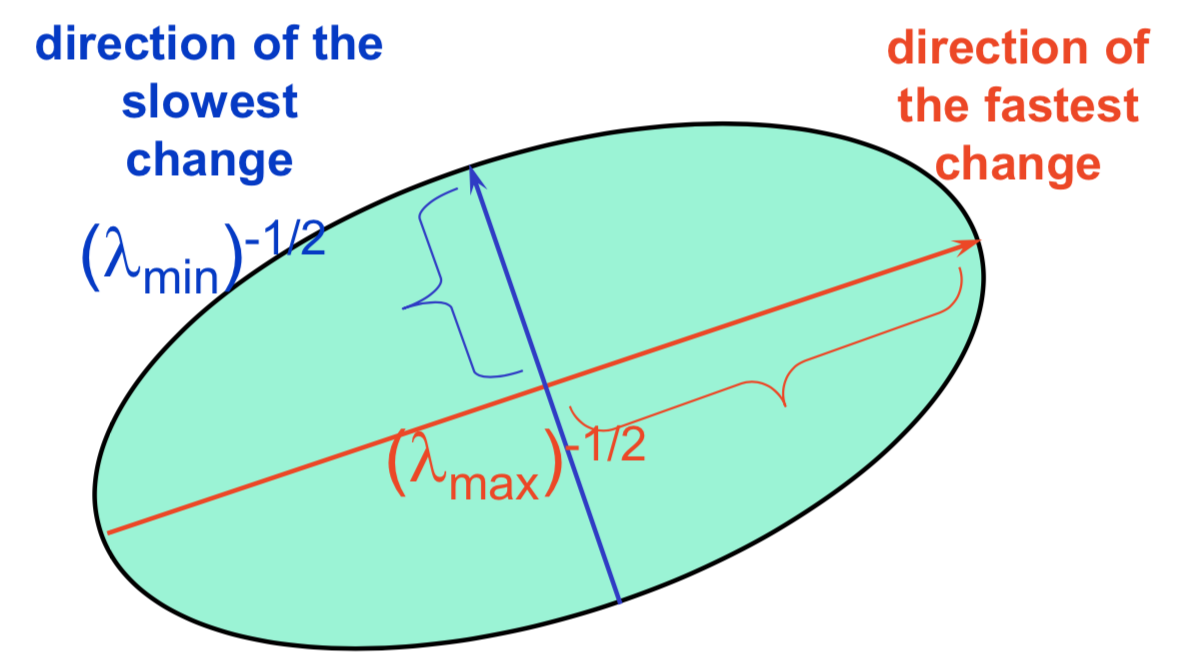
\includegraphics[width=0.25\textwidth]{figures/cv_image_processing_harris_ellipse.png}
		\caption{Visualization of relation between eigenvalues and gradients.}
		\label{fig:cv_image_processing_harris_ellipse}
	\end{figure}
	% cv_image_processing_harris_ellipse.png
	\item If we have an edge, one eigenvalue is considerably greater than the other as in one direction we have a large gradient, whereas in the other (90 degrees) the pixels stay the same. Here, $R$ is smaller than 0 as $\lambda_1\lambda_2$ is small but $\lambda_1 + \lambda_2$ is large.
	\item Thus, we only have a corner if in both directions we have a (equally) high change. In that case, $R$ is positive as $\lambda_1\lambda_2$ is large.
	\item Other properties of the Harris Corner detector
	\begin{itemize}
		\item Partial invariance to \textit{affine intensity} change. As only derivatives are used, a bias term $I+b$ does not influence result. When multiplying an image by a factor $I\cdot a$, we scale the eigenvalues and thus the cornerness as well. We therefore might only have to adapt the threshold.
		\item \textit{Rotation invariant} as only the ellipse rotates but the eigenvalues stay the same
		\item \textit{Scaling sensitive}: The Harris corner detector is sensitive to scale as it usually applies LoG/Derivatives of Gaussians for determining $I_x$ and $I_y$. To make the corner detector invariant to scale, we can apply multiple gradient filters with different values for $\sigma$ and stack them together (3D output instead of 2D). We then perform the detector on various scales, and take in the end the maximum response over scales for every pixel.
	\end{itemize}
	\item Applications
	\begin{itemize}
		\item \textit{Image stitching} as for combining separate photos into a panorama. We therefore detect interest points in all images, and try to match those (description by e.g. SIFT/histogram/...)
		\item \textit{Object recognition} by comparing local features that were found for a specific object with the ones from another image.
	\end{itemize}
\end{itemize}
\section{Object recognition}
\begin{itemize}
	\item Challenges in object recognition
	\begin{itemize}
		\item Huge dimensionality (large input size)
		\item Image formation process (see Section~\ref{sec:img_formation})
		\item Images are stationary signal and share features, but have to distinguish it from noise
	\end{itemize}
	\item Hard to define explicit rules, but easy to collect examples $\Rightarrow$ Machine learning
\end{itemize}
\subsection{Image representations}
\begin{itemize}
	\item Need to find an image representation that is able to capture the semantics of an image and hence makes it easy to recognize objects
	\item For normal pixel values, the euclidean distance does not reflect the similarity of images well. A change of illumination or translation has a huge impact on the metric although it is the same object
	\item Global histograms over whole image are scale and translation invariant, but are not really distinctive (different images have same histogram)
	\item The best way is to find \textit{local features} that images share. They are more descriptive and reoccur in different images. In the next step, we have to describe these features to get a final representation. 
	\item One way to describe them are using SIFT (Scale-invariant feature transform) which creates a local histogram of gradients in the neighborhood (see Figure~\ref{fig:SIFT})
	\begin{figure}[ht!]
		\centering
		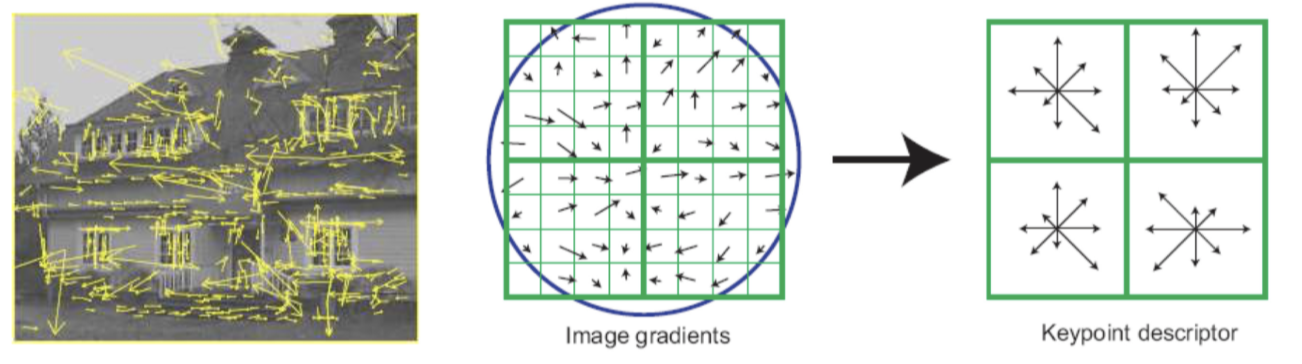
\includegraphics[width=0.6\textwidth]{figures/cv_object_detection_SIFT.png}
		\caption{SIFT descriptors for a $2\times 2$ histogram patch (normally $4\times 4$ see Figure~\ref{fig:descriptor_SIFT}).}
		\label{fig:SIFT}
	\end{figure}
\end{itemize}
\subsubsection{Histogram of Gradients (HoG)}
\begin{itemize}
	\item A HoG descriptor abstracts a patch by a histogram of gradient orientations. \item The steps for calculating a HoG descriptor for a given patch are
	\begin{enumerate}
		\item Determine pixel-wise gradients $I_x$ and $I_y$ by e.g. applying a Sobel filter (or rather simple $[1,-1]$ derivative filter)
		\item Determine the orientation $\theta = \arctan \frac{I_y}{I_x}$ and magnitude $I=\sqrt{I_y^2 + I_x^2}$ of the pixel-wise gradients
		\item Report gradients as a histogram. For example, if we take a 9 bin histogram, we map every gradient to the closest value of $0^{\circ}$, $45^{\circ}$, $90^{\circ}$ etc. Note that the 9th bin is for zero gradients which have no orientation.
	\end{enumerate}
	\item An improvement to simply counting the number of gradients is considering their magnitude as well, or using a non-hard counting ($30^{\circ}$ counts for $0^{\circ}$ and $45^{\circ}$).
	\item A disadvantage of HoG is that it is not rotational invariant
	\begin{figure}[ht!]
		\centering
		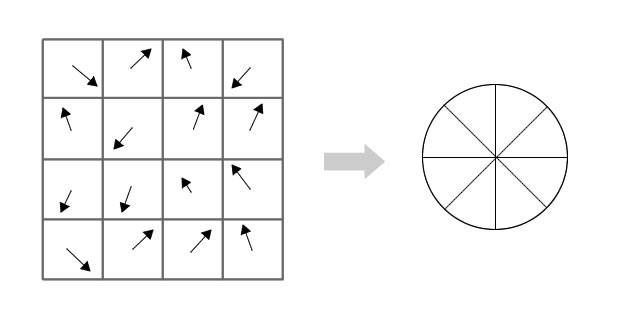
\includegraphics[width=0.4\textwidth]{figures/cv_image_processing_HoG.jpg}
		\caption{The HoG descriptor takes the gradients in a patch and group them into a histogram of orientations.}
		\label{fig:descriptor_HoG}
	\end{figure}
\end{itemize}
\subsubsection{Scale Invariant Feature Transform (SIFT)}
\begin{itemize}
	\item SIFT is a combination of detector and descriptor which is (mostly) both rotation and scale invariant
	\item The first step of SIFT is getting a scale-invariant response map. This is done by extracting features by LoG (or rather DoG due to runtime) on various scales (see Figure~\ref{fig:SIFT_scale_invariance})
	\begin{figure}[ht!]
		\centering
		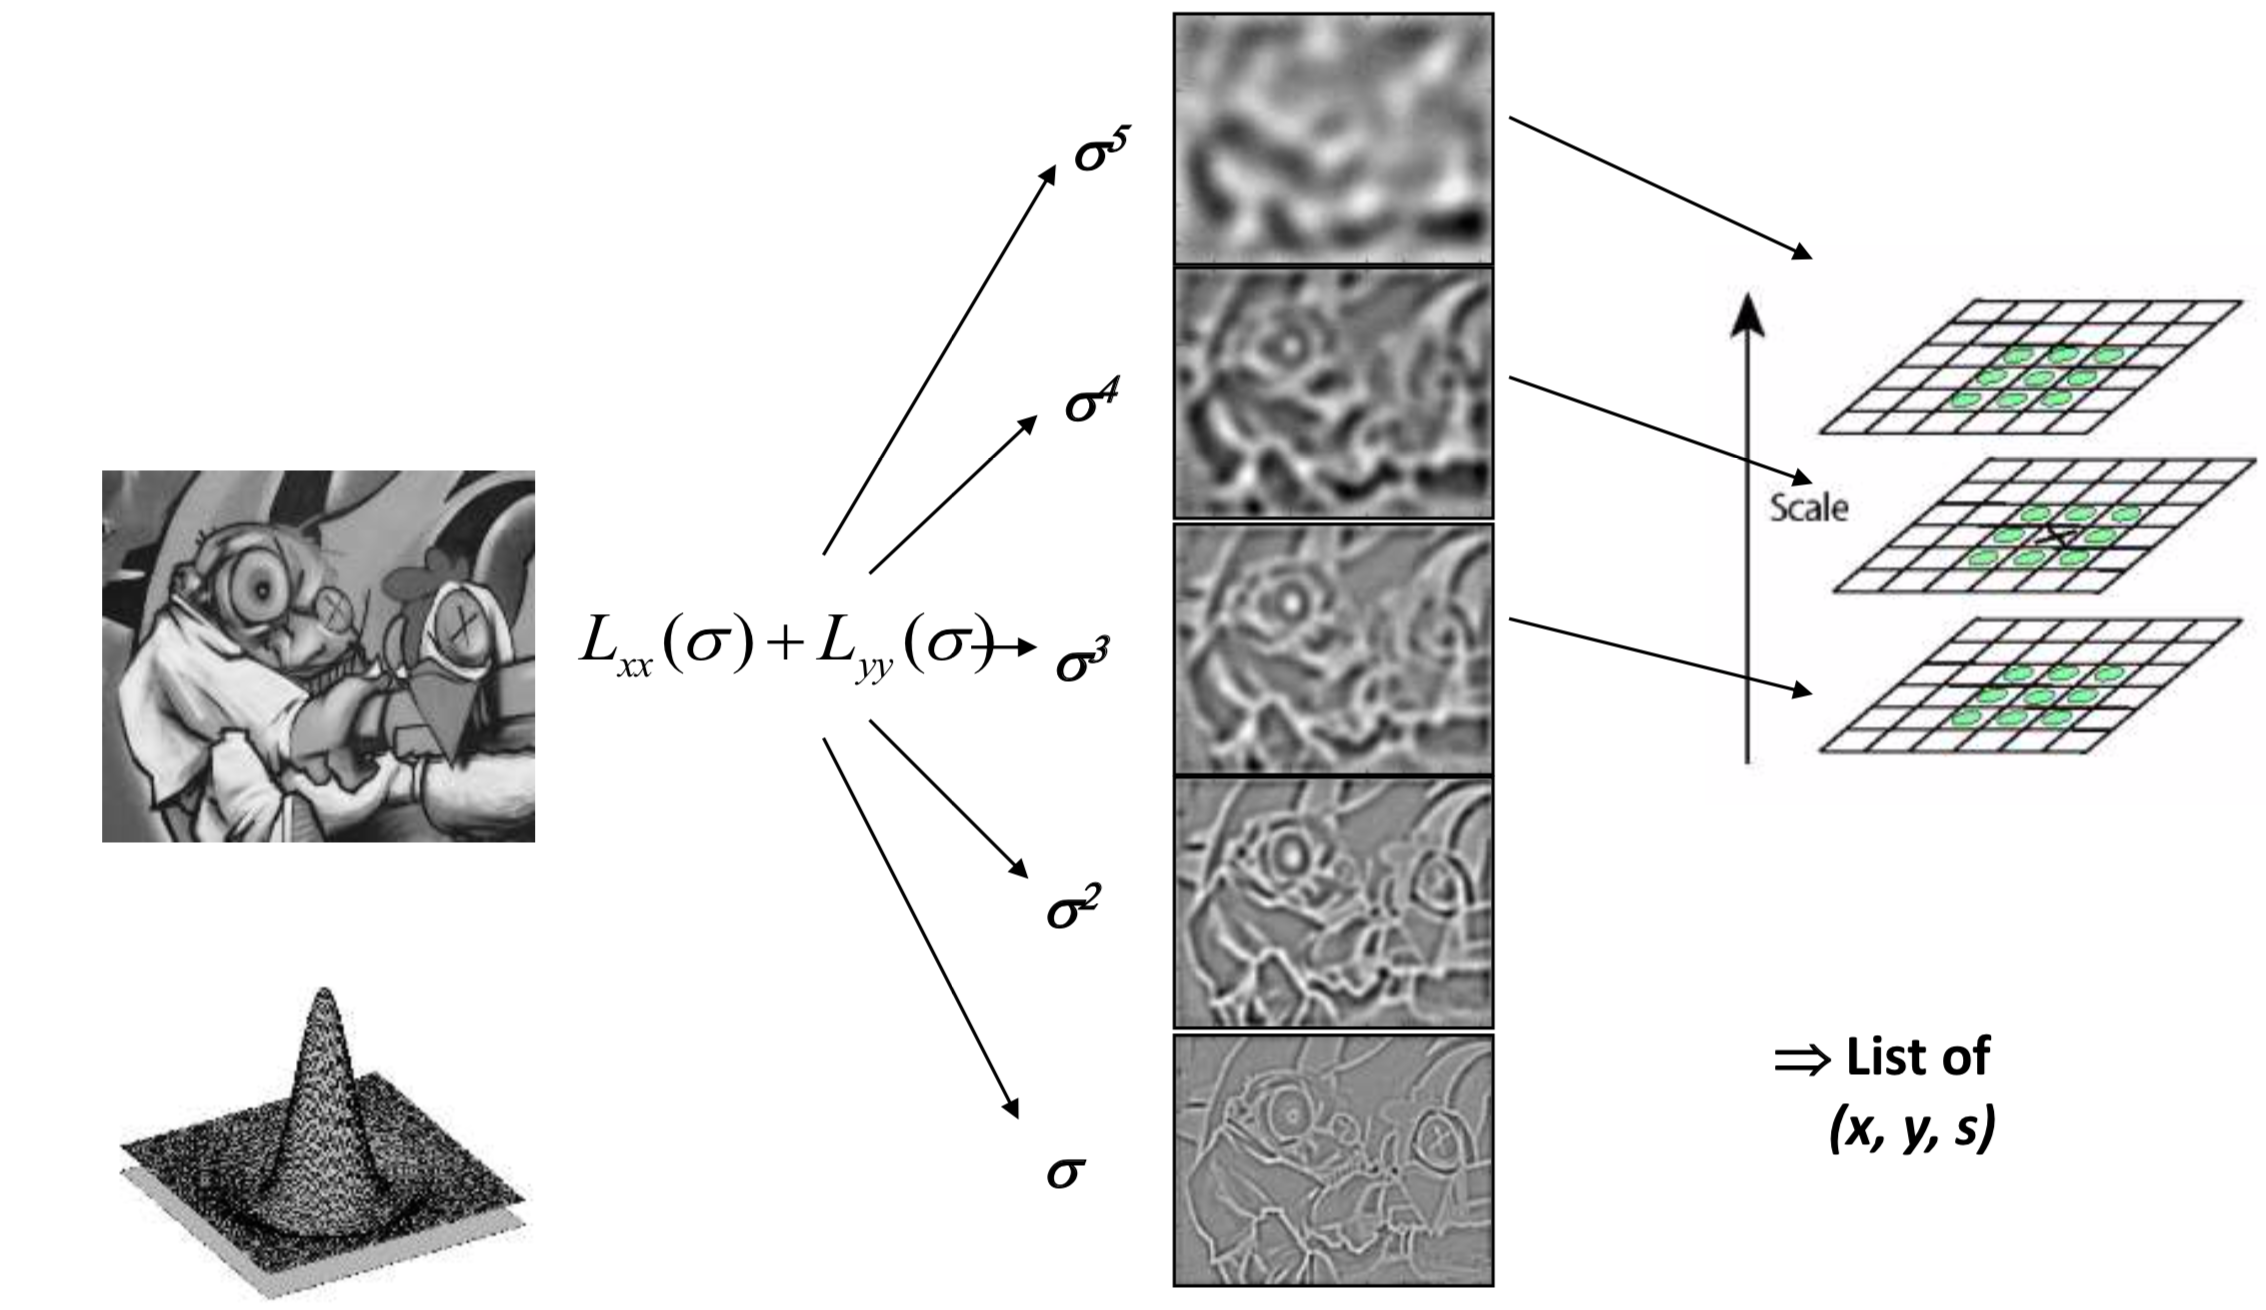
\includegraphics[width=0.5\textwidth]{figures/cv_image_processing_SIFT_scales.png}
		\caption{SIFT}
		\label{fig:SIFT_scale_invariance}
	\end{figure}
	\item We now look for local maxima in terms of both scale and location. This means that we search for points that are higher than all neighboring pixels in $x$-$y$ direction and scale (see Figure~\ref{fig:SIFT_scale_invariance} green points on the right) $\Rightarrow$ non-maximum suppression
	\item Given these points, we check for their \textit{cornerness}. Only at those points, we need to calculate the gradients and estimate the eigenvalues:
	$$\frac{\text{Tr}(\bm{H})^2}{\text{Det}(\bm{H})} < \frac{(r+1)^2}{r}$$
	The term $(r+1)^2/r$ is just a new threshold that specifies the required ratio between first and second eigenvalue.
	\item To guarantee rotation invariance, we look for the dominant gradient orientation in the patch. This is done by creating a weighted histogram of gradient orientations in the whole patch (weighted by the magnitudes of these gradients), and take the orientation with the highest value as orientation of the patch. If the patch has other orientations that have a value of at least 80\% of the dominant orientation, we create another descriptor for those as well.
	\item Once a point is selected as a key-point, we can group all gradients in small regions in a histogram and combine them into a $4\times 4$ grid of histograms. Note that we adjust all gradients according to the orientation of the key-point. Our final descriptor has then 128 features ($4\times 4$ histograms with each $8$ bins, see Figure~\ref{fig:descriptor_SIFT})
	\begin{figure}[ht!]
		\centering
		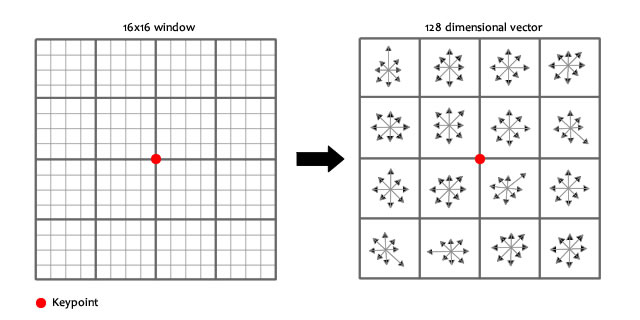
\includegraphics[width=0.5\textwidth]{figures/cv_image_processing_SIFT.jpg}
		\caption{A SIFT descriptor with $4\times 4$ histogram patch.}
		\label{fig:descriptor_SIFT}
	\end{figure}
\end{itemize}
\subsection{Bag-of-Words}
\begin{itemize}
	\item One approach for image representation is the visual Bag-of-Words (BoW). We therefore split an image into patches, describe each of these patches by one "visual word" (patch in our dictionary), and finally create a histogram out of it (see Figure~\ref{fig:BoW_pipeline})
	\begin{figure}[ht!]
		\centering
		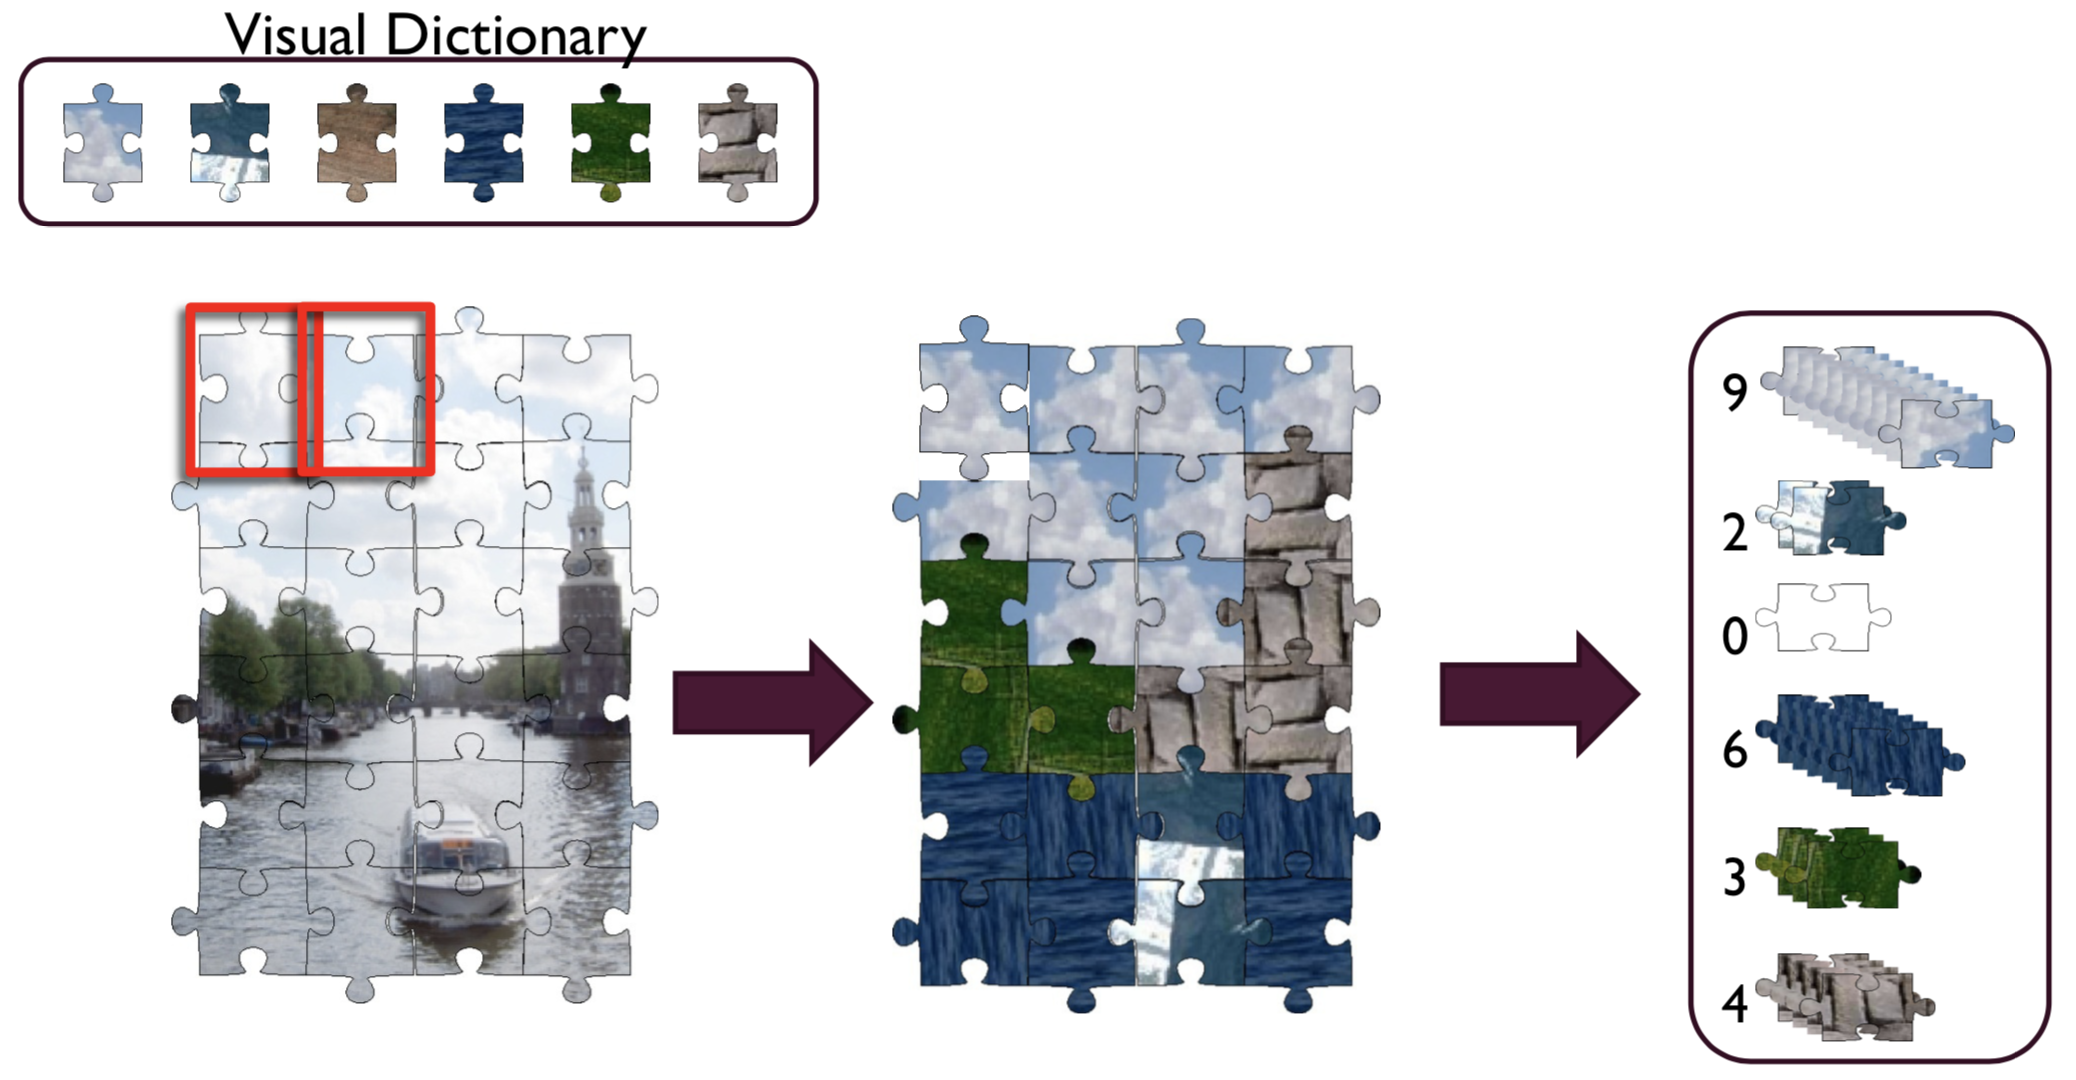
\includegraphics[width=0.5\textwidth]{figures/cv_object_detection_BoW_pipeline.png}
		\caption{General pipeline for BoW approach.}
		\label{fig:BoW_pipeline}
	\end{figure}
	\item There are four components of BoW for which a design choice has to be made
	\begin{itemize}
		\item \textbf{Patch sampling}: which patches should be used to describe an image. Can be either descriptive patches/interest points, but then the number of patches can significantly differ from image to image. Alternatively, we can perform a grid-like selection of patches (\textit{dense sampling}) on multiple scale (reduce size of image and sample again).
		\item \textbf{Patch description}: describe the patches/visual words by SIFT, RGB, HOG or similar. Goes along with image representation 
		\item \textbf{Visual dictionary}: create a dictionary by sampling a lot of patches from a large set of images (training images), and cluster them in their descriptor space to find distinctive patches. Use these clusters as visual words. There are different cluster methods that can be applied. However, one hyper-parameter is usually the number of clusters. High number of clusters give very distinctive, but noise sensitive patches, whereas low number of clusters give general, but less distinctive patches.
		\item \textbf{Histogram creation}: the simplest approach is finding the nearest prototype/visual word for every sampled batch of the image by e.g. L2 on the descriptor, and record the number of occurrences for each visual word. There are many (more advanced) alternatives that for example take the distance to the cluster means into account, or calculating mean and stddev etc. 
	\end{itemize} 
	\item Advantages and drawbacks of visual BoW
	\begin{itemize}
		\item[+] Translation invariant
		\item[+] Fixed length feature vector 
		\item[$-$] Loss of spatial information
		\item[$-$] Quantization loses information (mapping to visual words)
	\end{itemize}
	\item In order to keep some spatial information, we can extend the histogram by using multiple scales (spatial pyramid) and concatenate those for an output feature vector. Another approach would be to use the spatial information ($xy$-position) as additional features for the patch descriptor, and use during matching/clustering.
	\begin{figure}[ht!]
		\centering
		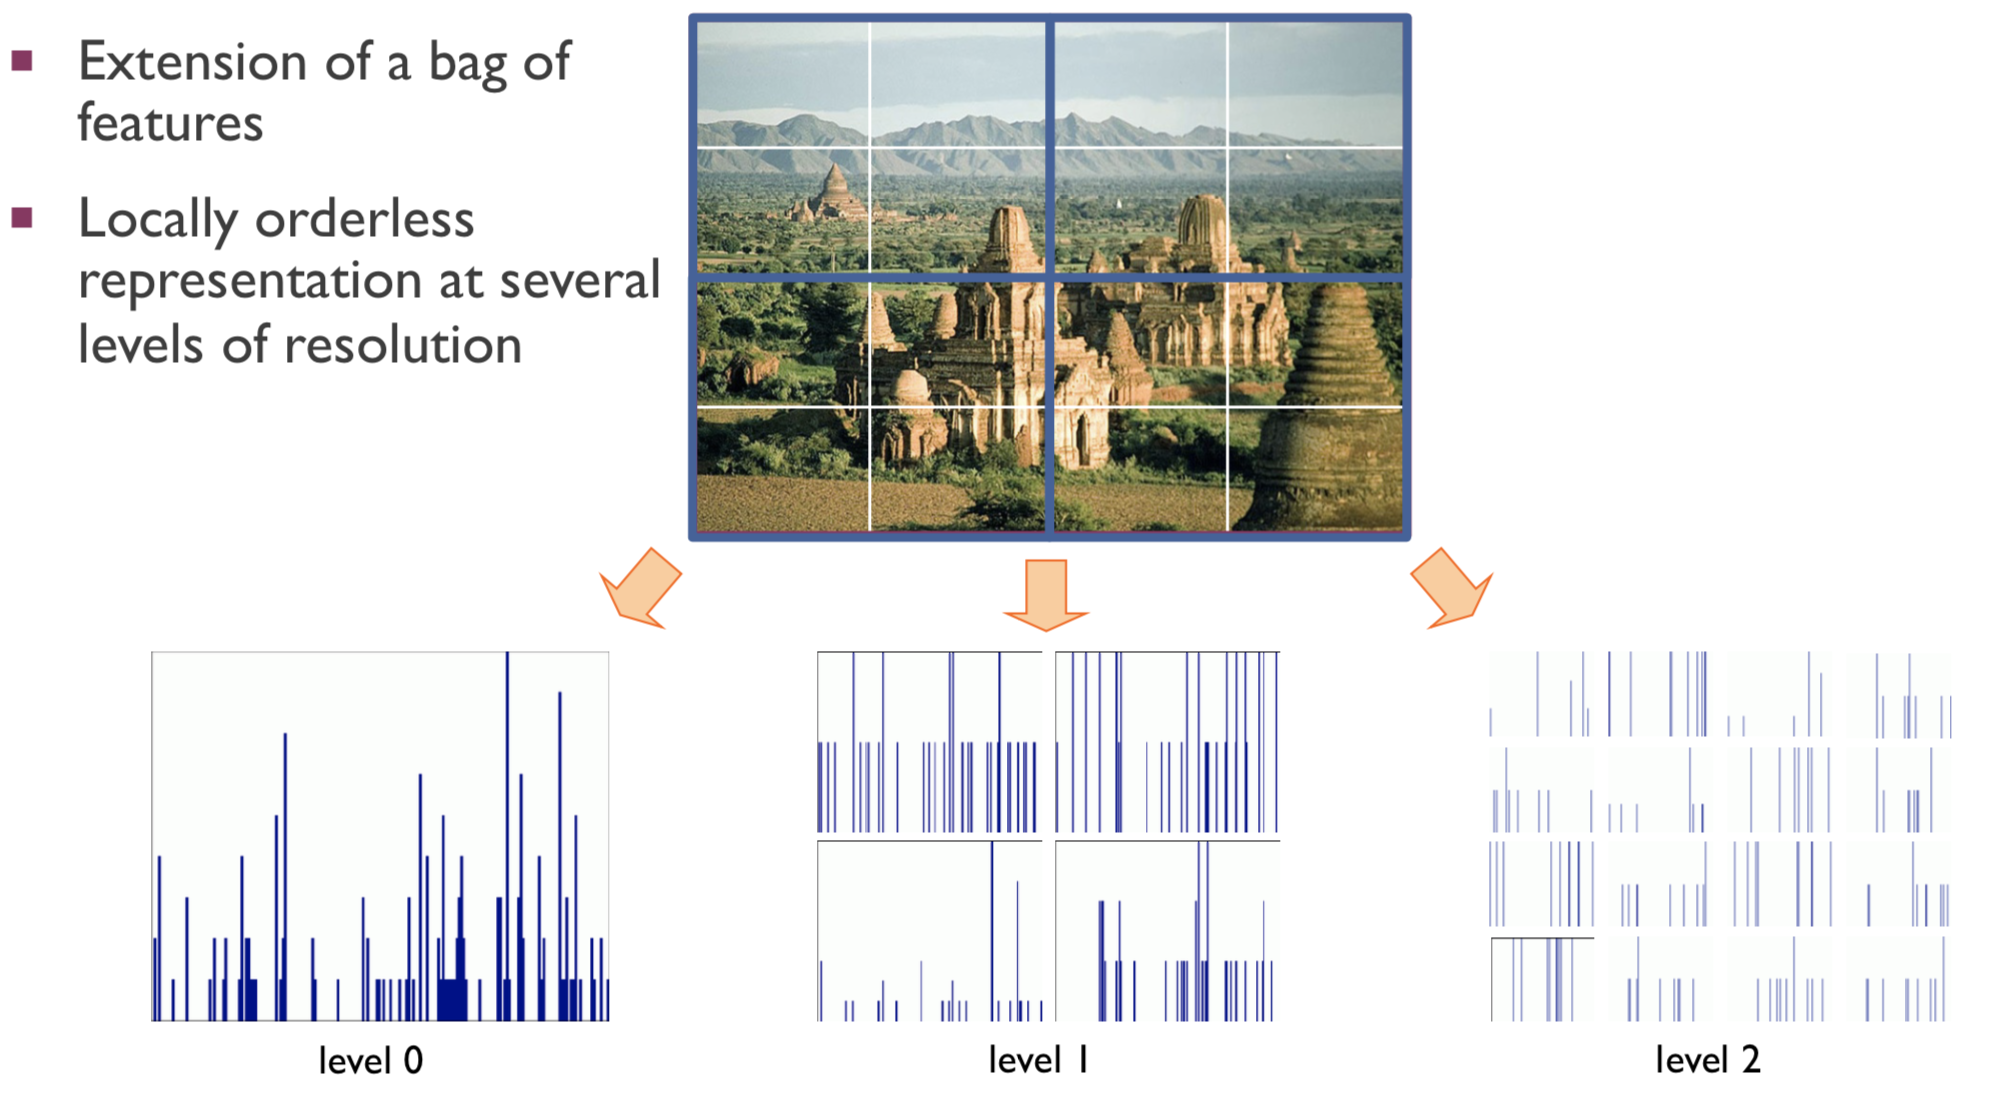
\includegraphics[width=0.45\textwidth]{figures/cv_object_detection_BoW_spatial_pyramid.png}
		\caption{Spatial pyramid for histogram creation. We concatenate all histogram to a longer feature vector.}
		\label{fig:BoW_spatial_pyramid}
	\end{figure}
\end{itemize}
\subsubsection{Bag of Words for Retrieval}
\begin{itemize}
	\item We can compare images for the retrieval task by their BoW histogram. This is more efficient and faster than checking for every interest point and try to compare those.
	\item Offline, we have to create the BoW vocabulary and determine a histogram for every image in our database
	\item When an image is entered as a query, we need to represent it by its BoW histogram and then compare it with every other.
	\item We can apply other techniques from IR as well like TF-IDF, query expansion, stop word removal, inverted file index,...
	\item To guarantee a good performance for the first retrieved examples, we can rerank the top $k$ by using geometrical verification (detect interest points and try to match those)
\end{itemize}
\subsection{Object detection}
\begin{itemize}
	\item Localization of objects in an image. Often approximated by bounding boxes that should be predicted around the object.
	\item A simple sliding window approach is too expensive as it generates 1) a lot of boxes over 2) a lot of scales with 3) different box ratios/shapes and 4) many classes.
	\item Hence, the first challenge is to find a set of relevant boxes with ``object'' (also called \textit{candidate boxes} all graded by an objectness score), and in a second step determine the class of the object in this candidate boxes
	\item One approach for that is \textbf{selective search} which is based on the property of images being hierarchical
	\begin{itemize}
		\item Segment image into small fragments based on simple approaches. Generate for all of these a candidate box
		\item For multiple iterations (recursively), combine two fragments that are the most similar together and consider a box for the combined fragment as well. Repeat until only one region is left
		\item Apply a classifier on those candidate boxes
	\end{itemize}
	\item A general pipeline for object detection is shown in Figure~\ref{fig:cv_object_detection_BB_pipeline}
	\begin{figure}[ht!]
		\centering
		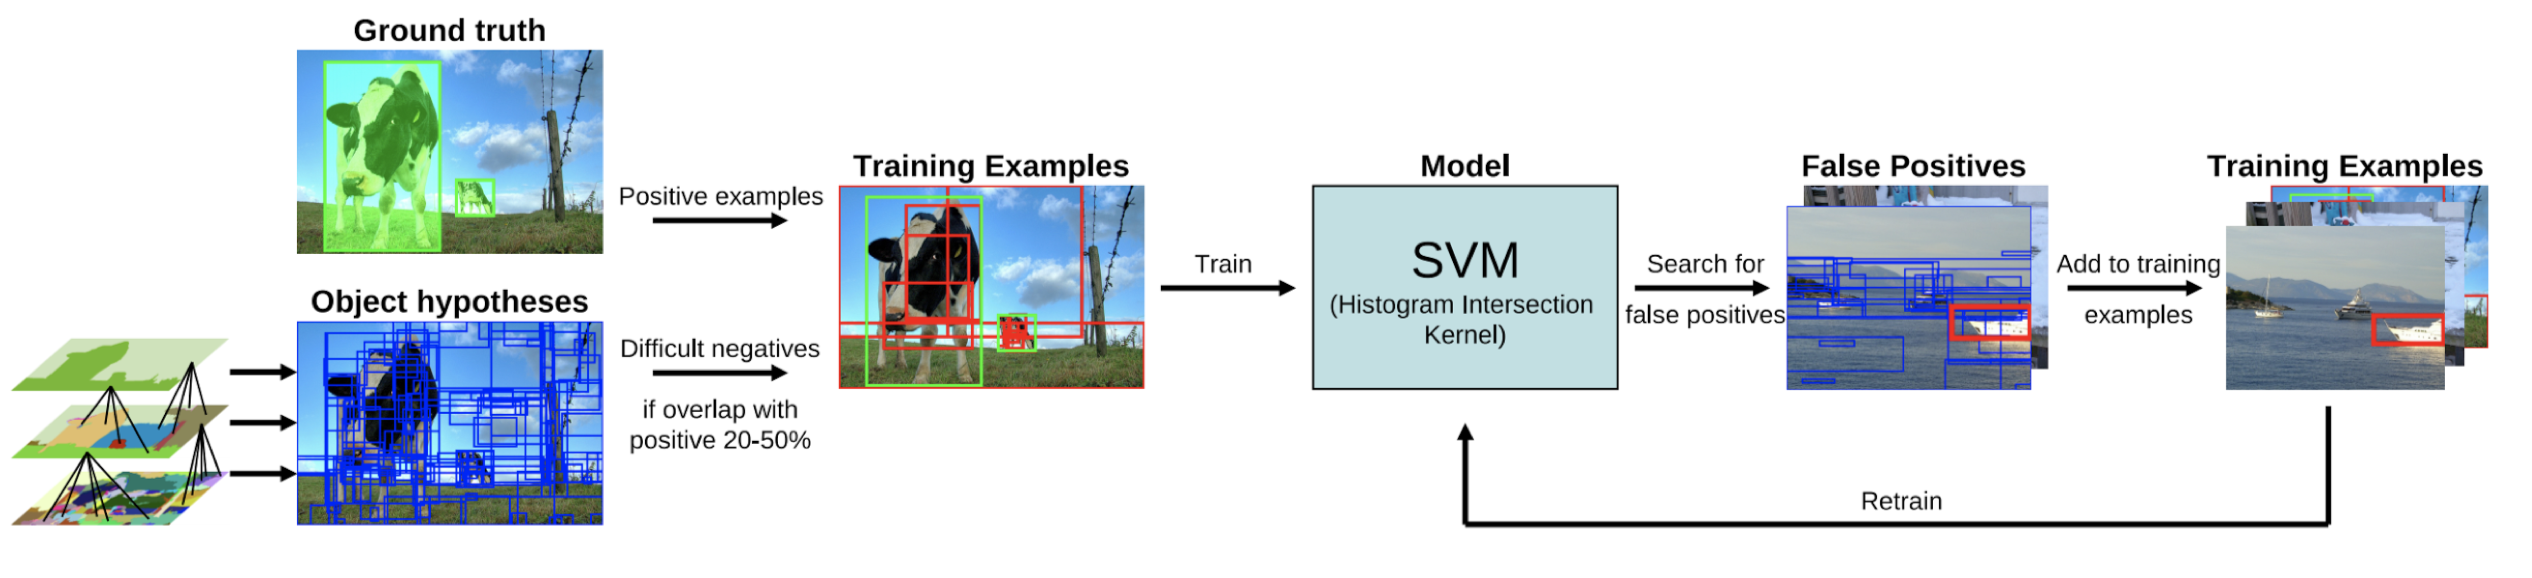
\includegraphics[width=0.45\textwidth]{figures/cv_object_detection_BB_pipeline.png}
		\caption{Pipeline for object detection with Bounding Boxes1.}
		\label{fig:cv_object_detection_BB_pipeline}
	\end{figure}
	% cv_object_detection_BB_pipeline.png
\end{itemize}
\section{Deep Learning}
\begin{itemize}
	\item Deep Neural Networks perform hierarchical feature learning and classification in a single architecture
\end{itemize}
\subsection{Convolutional Neural Networks}
\begin{itemize}
	\item Key layer of CNNs are convolutions. The weights are surface-wise local, but depth-wise global.
	\item Multiple neurons look at the same position, but using different kernels (channels)
	\item Parameters of a convolutional layer
	\begin{itemize}
		\item \textit{Kernel size}: size of the filter which is learned. If size is $k\times k$, we learn overall $k^2$ parameters per channel
		\item \textit{Input channels}: number of input channels $c_i$. Every filter has the size of $k\times k\times c_i$
		\item \textit{Output channels}: number of output channels $c_o$. Represent the number of different filters learned.
		\item \textit{Stride} with which we slide the filter over the image. Stride of $s=1$ means we apply a filter on every pixel as usual, $s=2$ would skip every second pixel and $s=4$ takes only every fourth pixel as center of an filter application. Default: $s=1$.
	\end{itemize}
	\item Overall, we learn $(k\times k\times c_i + 1)\times c_0$ \textbf{parameters} in a convolutional layer (the 1 extra parameter for bias)
	\item The \textbf{output size} is calculated by $$h_o = (h_i + 2\cdot p - k) / s + 1$$ where $p$ is the padding (number of extra pixels on each side)
	\begin{figure}[ht!]
		\centering
		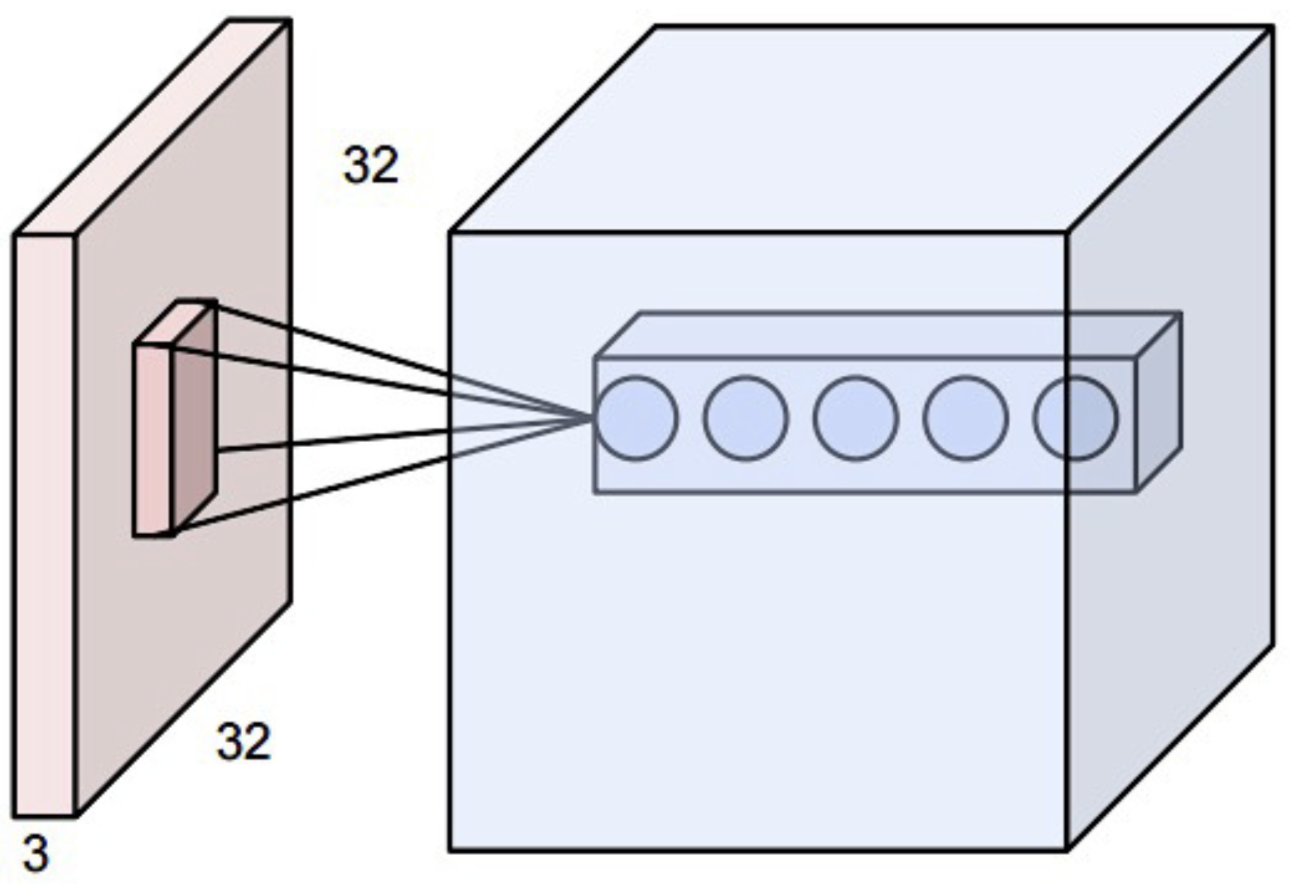
\includegraphics[width=0.2\textwidth]{figures/cv_deep_learning_convolution_operator.png}
		\caption{Convolutional layer in a CNN}
	\end{figure}
	\item Activation layers like ReLU ($\max(0,x)$) introduce non-linearity
	\item Pooling aggregates multiple values into a single value making it invariant to small transformations. Reduces the size of the next output layer while keeping the most important information 
\end{itemize}
\subsubsection{Transfer Learning}
\begin{itemize}
	\item Reuse information gained on a large dataset (e.g. ImageNet) on a new one
	\item Depending on the amount and similarity of data with the pretrained one, we should fine-tune different layers (see Figure~\ref{fig:transfer_learning})
	\item Transfer Learning can greatly influence the performance of a network. Low level features (first layers) are almost always the same for images as we have to detect edges, colors, etc.
\end{itemize}
\begin{figure}[ht!]
	\centering
	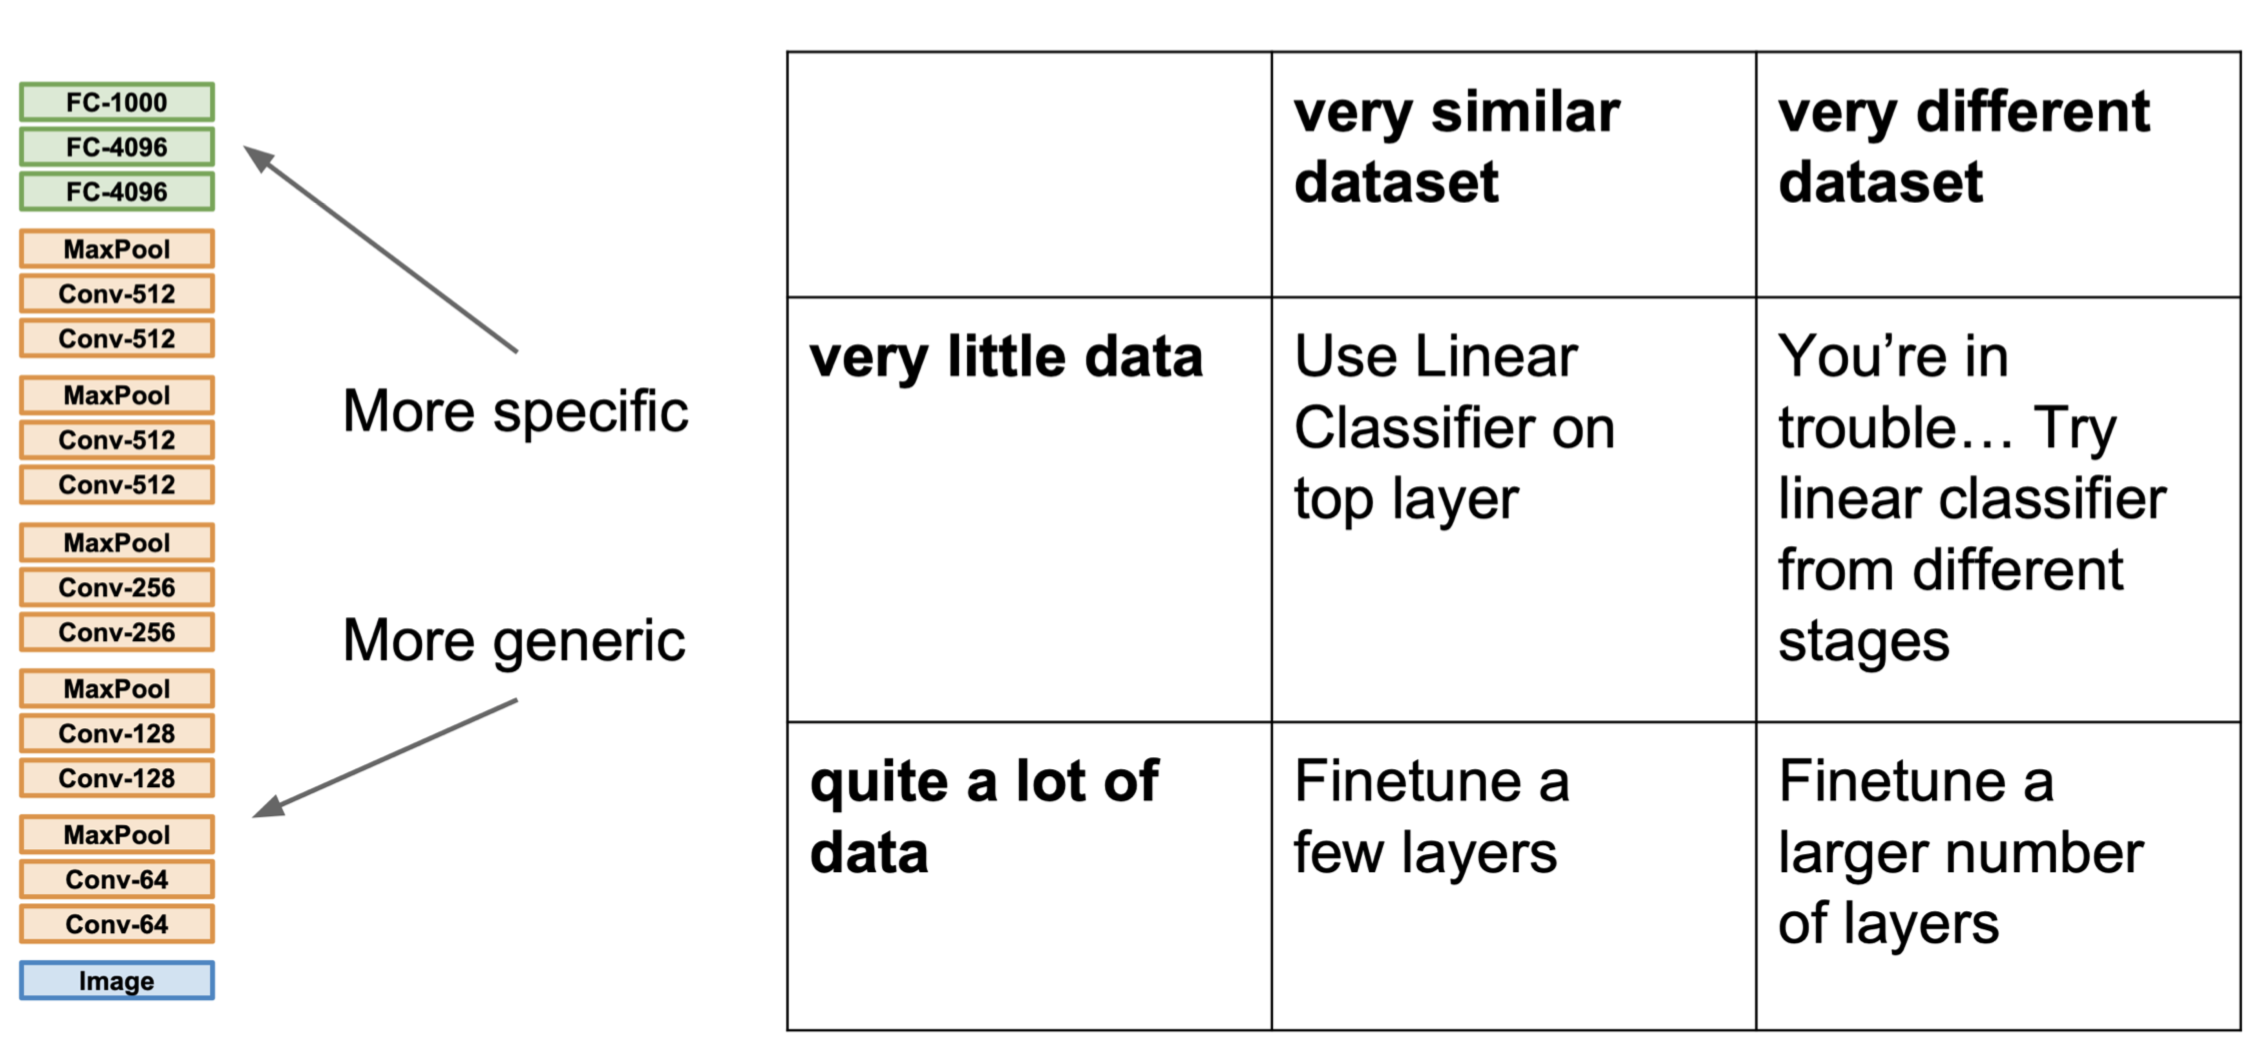
\includegraphics[width=0.5\textwidth]{figures/cv_deep_learning_transfer_learning.png}
	\caption{Transfer learning}
	\label{fig:transfer_learning}
\end{figure}
% cv_deep_learning_transfer_learning.png
\subsection{GANs}
\begin{itemize}
	\item Capture the underlying data distribution and being able to generate new samples
	\item Next to generative adversarial networks, we can also apply Variational Autoencoders or PixelCNN/RNN for this task
	\item GANs are trained by a minimax game between two neural networks (Discriminator $D$ and Generator $G$). $G$ wants to fool $D$ by generating realistic images. $D$ tries to distinguish between generated and real images/data:
	$$\min_G \max_D V(G,D) = \mathbb{E}_{\bm{x}\sim p_{\text{data}}(\bm{x})} \left[\log \left(D\left(\bm{x}\right)\right)\right] + \mathbb{E}_{\bm{z}\sim p_{z}(\bm{z})} \left[\log\left(1 - D\left(G\left(\bm{z}\right)\right)\right)\right] $$
	\item The standard/plain GAN architecture uses a noise vector $\bm{z}$ as input to the generator. Note that it is also possible to put  and condition the GANs input on the output (aka \textit{conditional GANs}). To ensure that the generator learns a relation from input to output, we might need to add an additional loss term like MSE to a label
	\item The training procedure consists of two steps which can be alternated or repeated by themselves for multiple times
	\begin{enumerate}
		\item \textit{Fix $G$ and train $D$}: in order to train the discriminator, we let $G$ generate fake images and feed the discriminator both the fake and sampled real data. Note that we need to fix $G$ to not backpropagate the error of $D$ through $G$.
		\item \textit{Fix $D$ and train $G$}: $G$ is trained by generating images and backpropagating the error of the prediction of $D$ (towards prediction of a real image). Although the gradients flow back through $D$, we do not update any weights of the discriminator as we otherwise cheat (train $D$ to optimize loss of $G$)
	\end{enumerate}
\subsubsection{Stability and Training problems}
	\item In general, it is hard to train a GAN. There are a lot of problems that can occur
	\item \textbf{Vanishing gradients} during training:
	\begin{itemize}
		\item If the discriminator is too bad, the generator does not get valid/accurate feedback and can therefore not learn properly
		\item If the discriminator is perfect, the generator has very low gradients as a small change does not influence the discriminator
		\begin{figure}[ht!]
			\centering
			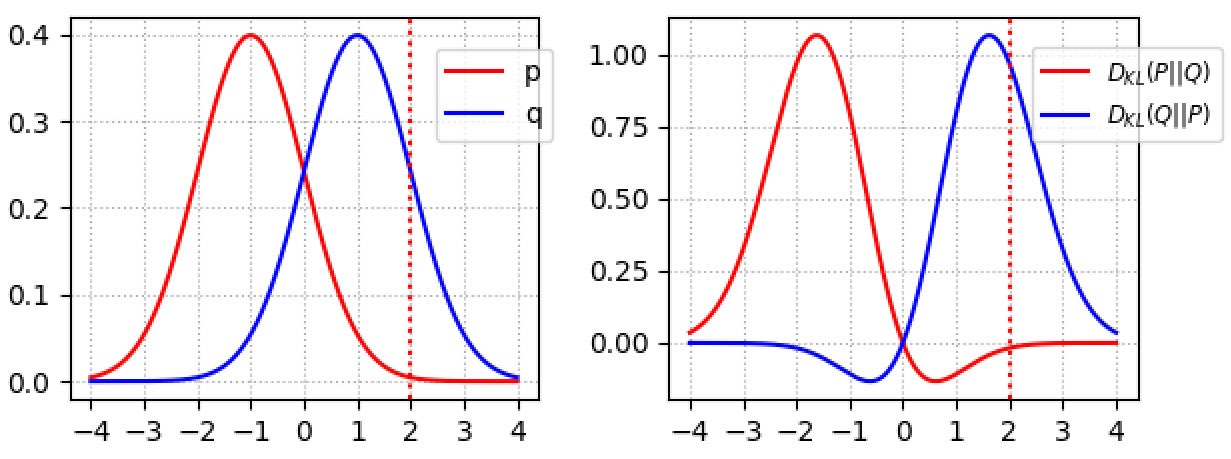
\includegraphics[width=0.4\textwidth]{figures/cv_deep_learning_GAN_vanishing_gradients.jpeg}
			\caption{Vanishing gradients problem for training with KL-divergence. When the distance between the two distributions $p$ and $q$ (respectively $P_g$ and $P_r$) is too huge, the KL divergence is very close to zero. Hence, is does not provide any strong gradients in these regions.}
		\end{figure}
	\end{itemize}
	\item \textbf{Reaching the equilibrium}
	\begin{itemize}
		\item We know that the nash equilibrium of the minimax game is $P_g=P_r$ meaning the distribution of the real data is equal to the generated data. In that case, $D$ return 0.5 no matter what example we put in (as both distributions are equal).
		\item However, it has been shown that such cost functions may not converge when using gradient descent. An example is shown in Figure~\ref{fig:GAN_reaching_equilibrium}.
		\begin{figure}[ht!]
			\centering
			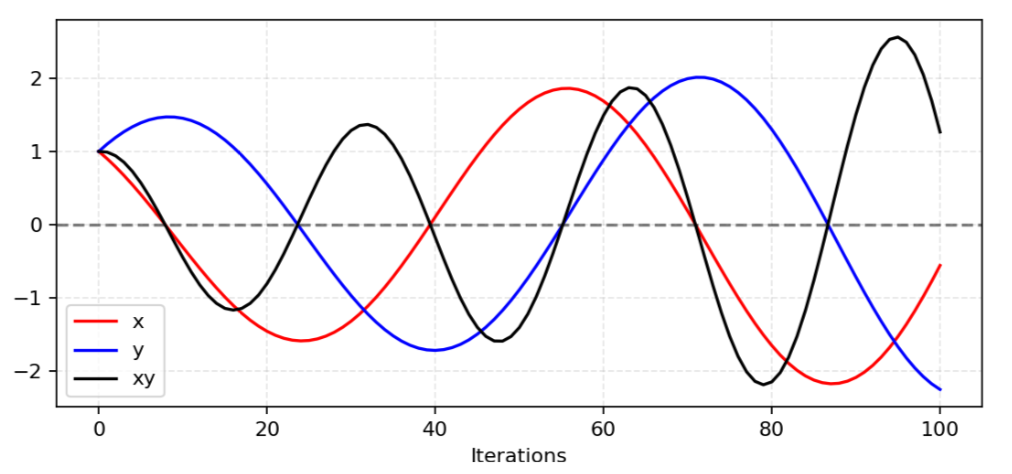
\includegraphics[width=0.4\textwidth]{figures/cv_deep_learning_GAN_oscillating.png}
			\caption{Oscillating behavior of a non-cooperative game where $\min_x \max_y V(x,y) = x\cdot y$. The equilibrium $x=y=0$ is never reached.}
			\label{fig:GAN_reaching_equilibrium}
		\end{figure}
	\end{itemize}
	\item \textbf{Mode collapse}
	\begin{itemize}
		\item A GAN suffers from a mode collapse if the generator limits its predictions/generated distribution to a few samples/modes.
		\item For example in case of the MNIST dataset, this would mean that the generator only creates numbers of one or two different digits. Although a full mode collapse is rarely the case, partial mode collapses frequently occur
		\item In order to create a mode collapse, the gradients regarding the noise $\bm{z}$ must be very low/close to zero. This can for example happen if we fix the discriminator and the generator converges to the optimal image $\bm{x}^*$ that fools the discriminator the most
		\item Once the generator collapse to one mode, the discriminator will learn that this mode is purely/mostly generated and thus changes its predictions. The generator will address that by changing the mode (note that as $\partial L/\partial \bm{z}\approx 0$, we will just collapse to the next mode and are not able to escape this loop).
		\item In the end, this turns into a cat-and-mouse game between the generator and discriminator, and will not converge (see Figure~\ref{fig:GAN_mode_collapse}).
		\begin{figure}[ht!]
			\centering
			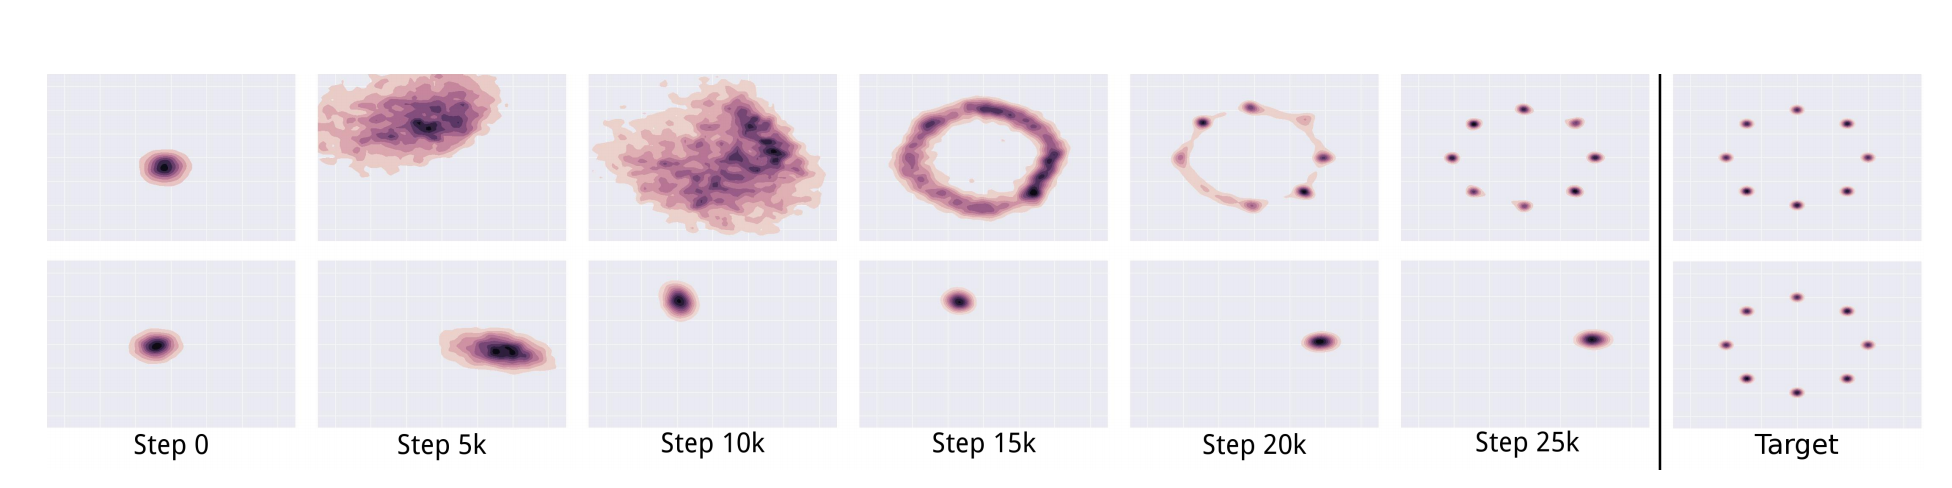
\includegraphics[width=0.6\textwidth]{figures/cv_deep_learning_GAN_mode_collapse.png}
			\caption{\textit{Top row}: optimal convergence of generator distribution to 8 modes. \textit{Bottom row}: Sample of a mode collapse after 10k iterations. The generator is only able to generate a single mode.}
			\label{fig:GAN_mode_collapse}
		\end{figure}
	\end{itemize}
\end{itemize}
\section{Deep Video}
\begin{itemize}
	\item Understanding a video requires to analyze spatial and temporal information. Thus, also more data is needed to fully train such a network whereas we cannot label every single frame (too expensive)
	\item Grid-like data can be processed by a CNN, temporal mostly by RNN, and for unstructured data a fully connected network is most suitable
	\item Easiest solution for video understanding would be to classify (sample/all) frames independently by standard CNN, and then perform average pooling over predictions. However, this approach does not capture temporal structure
\end{itemize}
\subsection{Recurrent Neural Networks}
\begin{itemize}
	\item In Recurrent Neural Networks, a hidden state flows over time steps. The vanilla RNN formula is
	\begin{equation*}
		\begin{split}
			h_t & = \tanh \left(W_{hh}h_{t-1} + W_{xh} x_{t}\right)\\
			y_t & = W_{hy} h_t
		\end{split}
	\end{equation*}
	\item Weights are shared over time (also $W_{hh}$) so that a RNN can process an arbitrary sequence length. Also, it reduces the number of parameters and thus the chance of overfitting 
	\item However, weight sharing can also lead to vanishing gradients as if we backpropagate from $h_t$ to $h_k$, we have a factor $\theta$ that lets the gradients vanish if it's lower than one, and explode if it is greater than one:
	$$\frac{\partial h_t}{\partial h_k} = \theta^{(t-k)} \sum f(\cdot)$$
	\item Vanilla RNNs have troubles capturing long-term dependencies. A possible solution is using LSTMs that control the information flow by three gates (see Figure~\ref{fig:deep_video_LSTM}):
	\begin{equation*}
		\begin{split}
			\text{Forget gate:  } & f_t = \sigma\left(W_f \cdot \left[h_{t-1}, x_t\right] + b_f\right)\\[7pt]
			\text{Input gate:  } & i_t = \sigma\left(W_i \cdot \left[h_{t-1}, x_t\right] + b_i\right)\\
			& \tilde{c}_t = \tanh\left(W_c \cdot \left[h_{t-1}, x_t\right] + b_c\right)\\
			& c_t = f_t * c_{t-1} + i_t * \tilde{c}_t\\[7pt]
			\text{Output gate:  } & o_t = \sigma\left(W_o \cdot \left[h_{t-1}, x_t\right] + b_o\right)\\
			& h_t = o_t * \tanh\left(c_t\right)
		\end{split}
	\end{equation*}
	\begin{figure}[ht!]
		\centering
		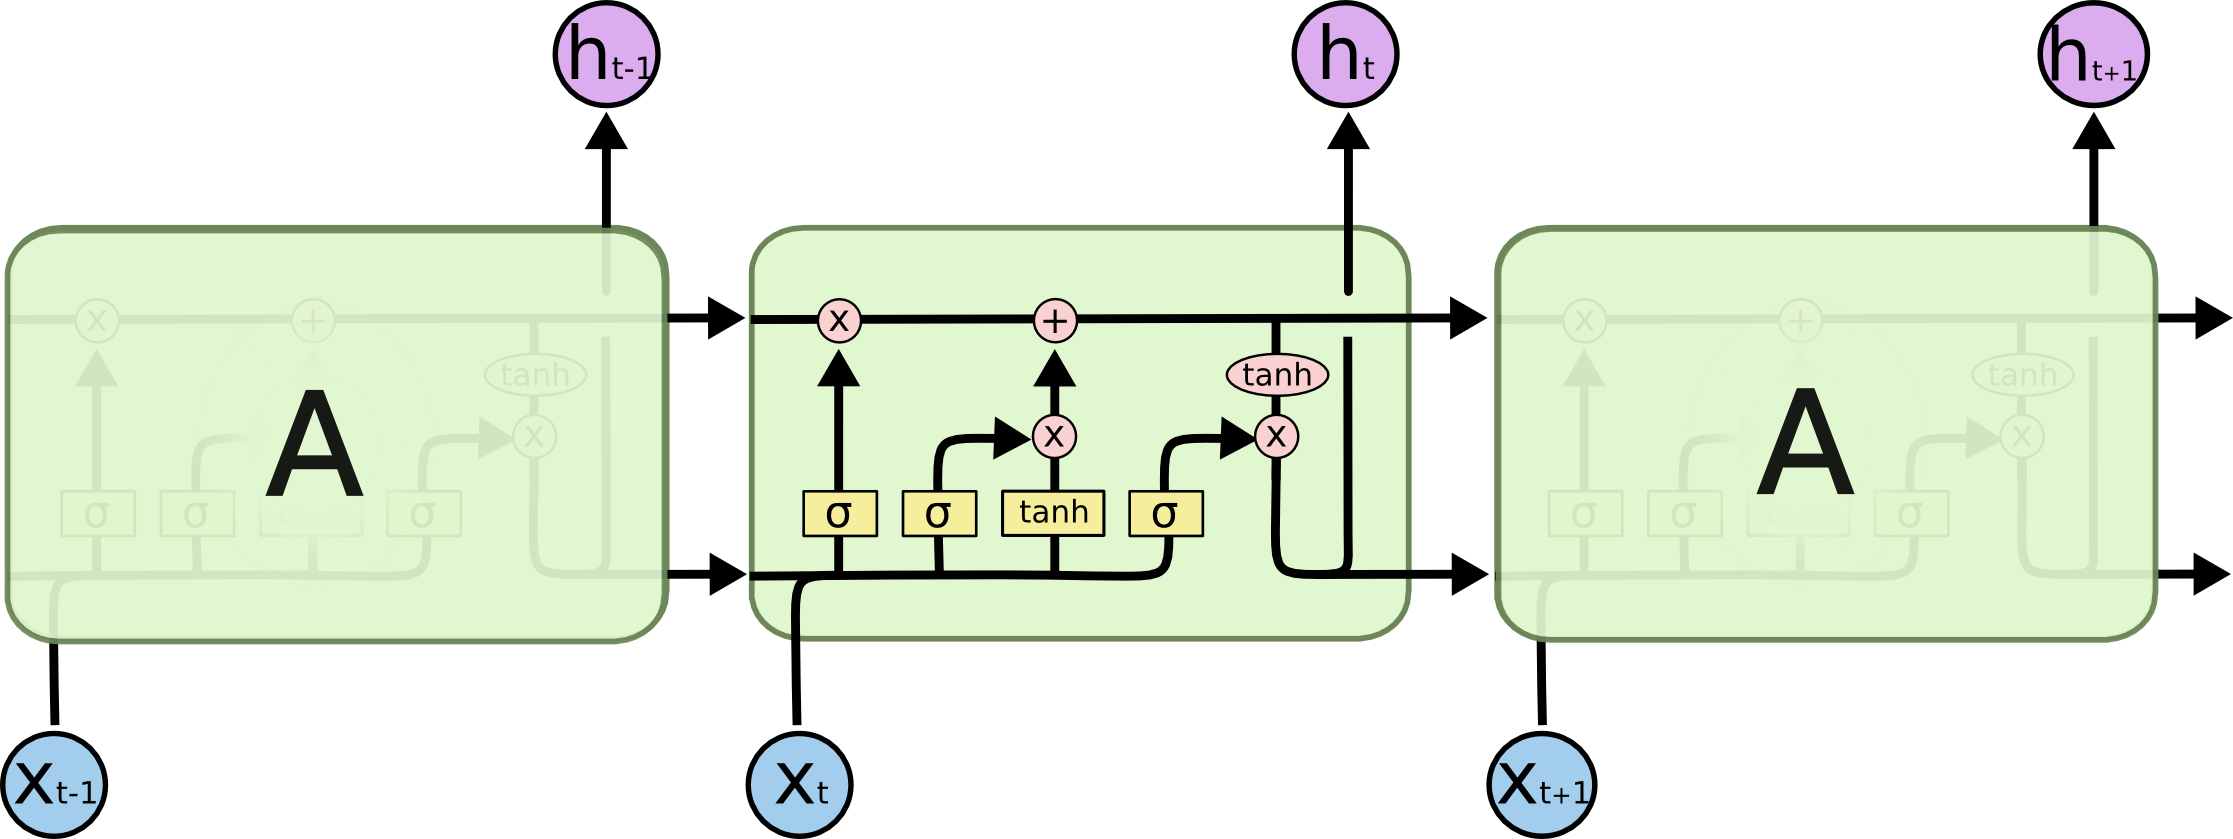
\includegraphics[width=0.5\textwidth]{figures/cv_deep_video_LSTM.png}
		\caption{Visual representation of a LSTM chain.}
		\label{fig:deep_video_LSTM}
	\end{figure}
\end{itemize}
\subsection{3D convolutions}
\begin{itemize}
	\item We can extend standard convolutions to 3D by moving the filter over the time dimension as well (channels are now 4th dimension over which filter is still global)
	\begin{figure}[ht!]
		\centering
		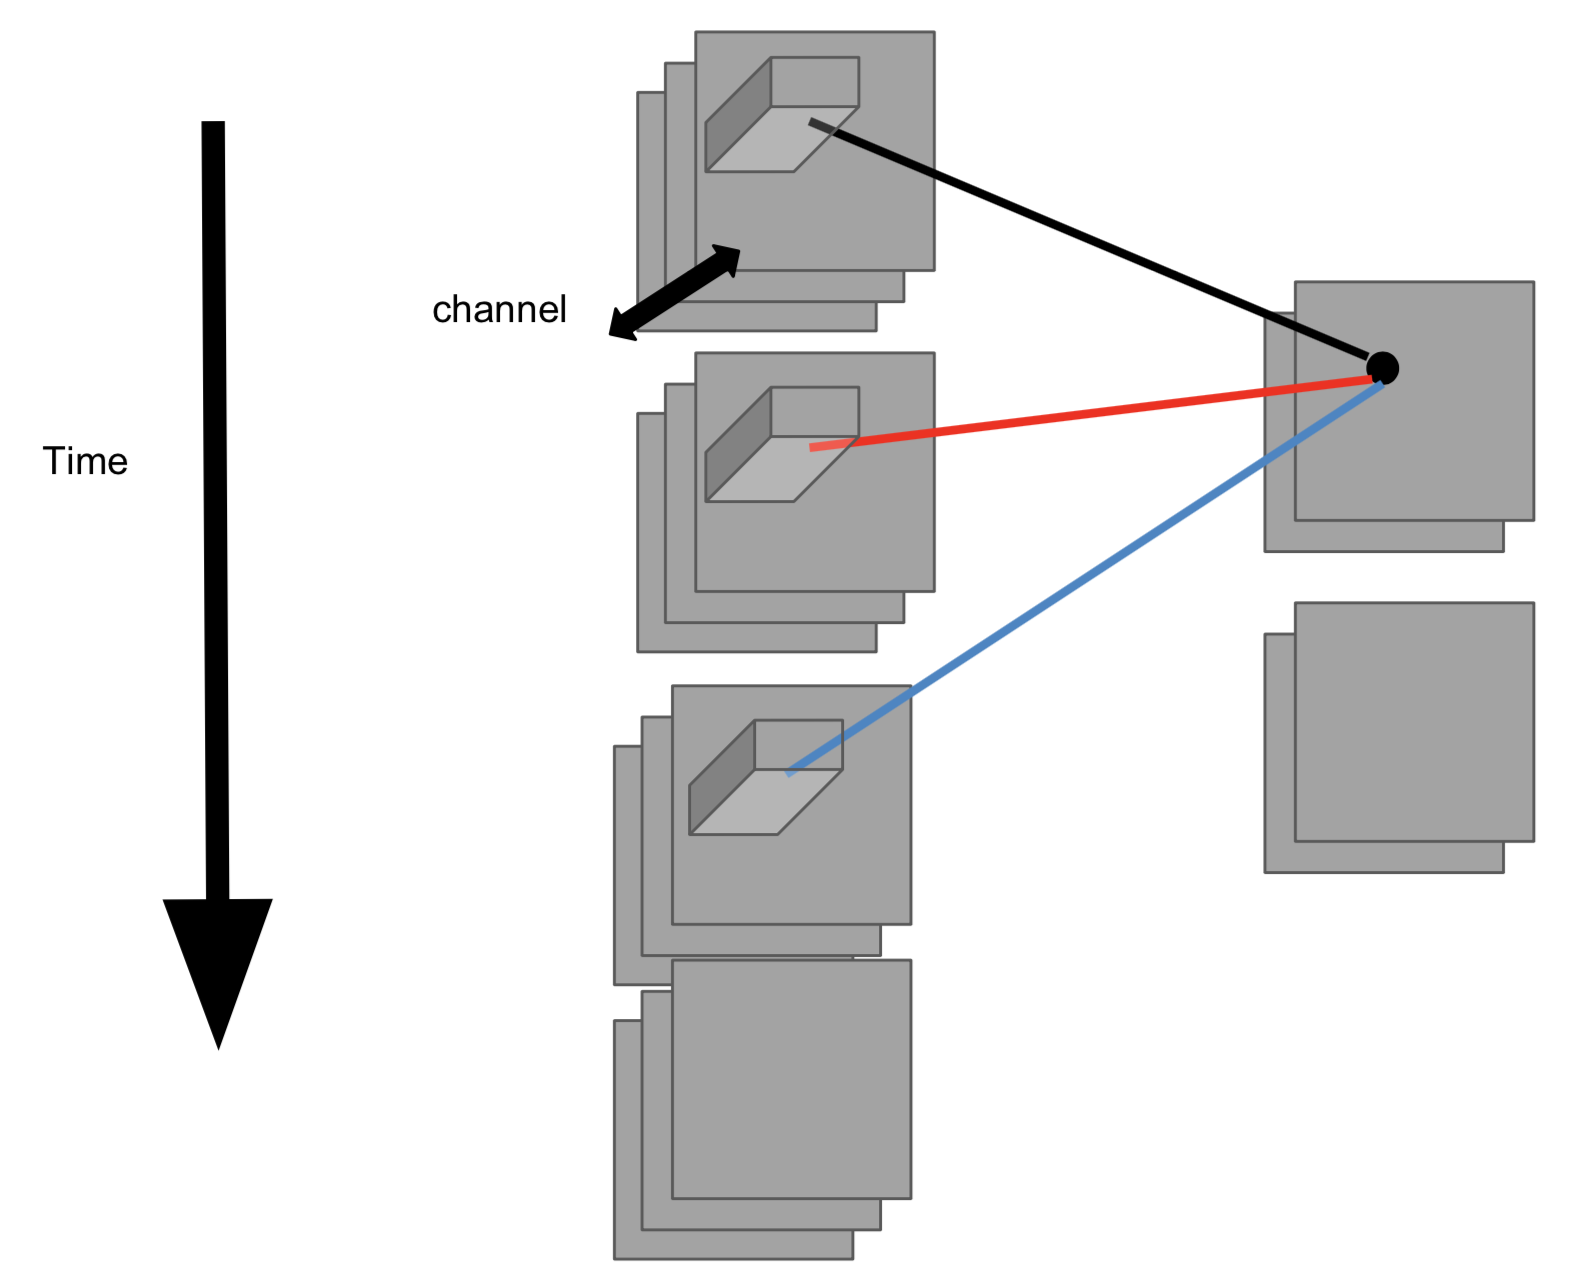
\includegraphics[width=0.3\textwidth]{figures/cv_deep_video_3D_convs.png}
		\caption{A 3D convolution is local over spatial and temporal dimensions, but still global over channels (i.e. RGB).}
		\label{fig:deep_video_3d_convs}
	\end{figure}
	\item Example: extending a 2D kernel by temporal dimension:
	\begin{equation*}
		\begin{split}
			200\times 200\times 3 \textcolor{blue}{\times 16} \xrightarrow{\text{filter }3\times3\textcolor{blue}{\times 3}} 200\times 200\times 256 \textcolor{blue}{\times 16}
			\Rightarrow \underbrace{3\times 3}_{\text{ spatial }}\underbrace{\textcolor{blue}{\times 3}}_{\text{ temporal }}\underbrace{\times 3}_{\text{ input channels }}\underbrace{\times 256}_{\text{ output channels}}\text{ parameters}
		\end{split}
	\end{equation*}
	\item Such convolutions learn combined temporal and spatial information. 
	\item Alternative is to concatenate all input frames over the channel dimension and pass it to a simple 2D network (also called \textit{early fusion}). Note that this approach loses the temporal information very fast
	\item Consecutive 3D convolutions can be seen as hierarchical combination of frames. Low level layers therefore capture low level motions, while high level layers (close to output) are able to reason about a longer set of frames and thus high level motion.
	\item Still, it is hard to learn long term dependencies with 3D convolutions as it does not have any gates and thus no explicit control over the information flow
	\item Note that in general, video-based networks are more likely to suffer from overfitting as the input space has a much higher dimensionality and the network has more parameters
\end{itemize}
\subsection{State-of-the-art}
\subsubsection{Two Stream Network}
\begin{itemize}
	\item Earliest proposed network for action recognition was \textbf{Two stream network}
	\item The architecture consists of two networks. One takes a single frame (\textit{spatial} stream net), and the other processes the concatenated optical flow over the set of frames (\textit{temporal} stream net). Both predictions are in the end combined
	\item The biggest problem here is that the spatial and temporal information is processed independently, and the very late fusion makes it impossible to reason about both
	\item Other disadvantages include a higher computational cost (two networks plus optical flow), only capturing short motion (early fusion of optical flow), noisy optical flow, and higher probability of overfitting due to number of parameters
	\item Approach can be slightly improved by repeatedly applying the network on small snippets of the network, and combining the prediction afterwards
	\begin{figure}[ht!]
		\centering
		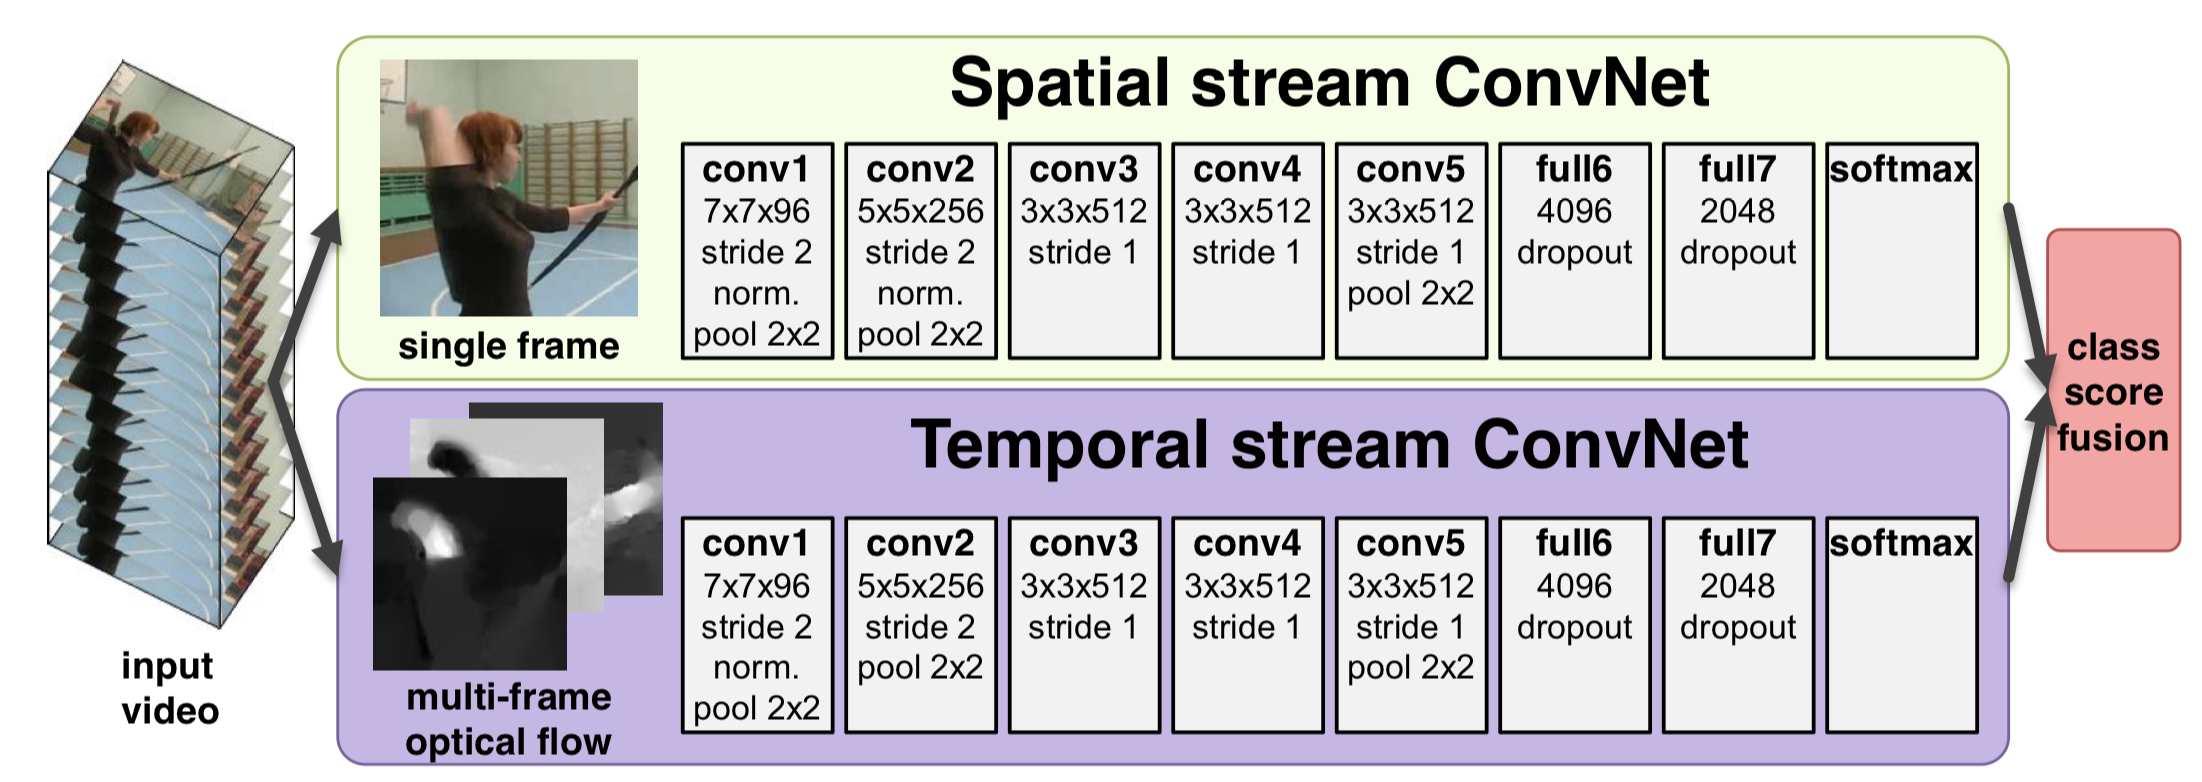
\includegraphics[width=0.5\textwidth]{figures/cv_deep_video_two_stream_network.png}
		\caption{Architecture of the two stream network.}
		\label{fig:deep_video_two_stream_net}
	\end{figure}
\end{itemize}
\subsubsection{I3D}
\begin{itemize}
	\item Inspired by the success of the 2D version (GoogLeNet), current state-of-the-art networks apply 3D inception modules (see Figure~\ref{fig:deep_video_I3D_module})
	\begin{figure}[ht!]
		\centering
		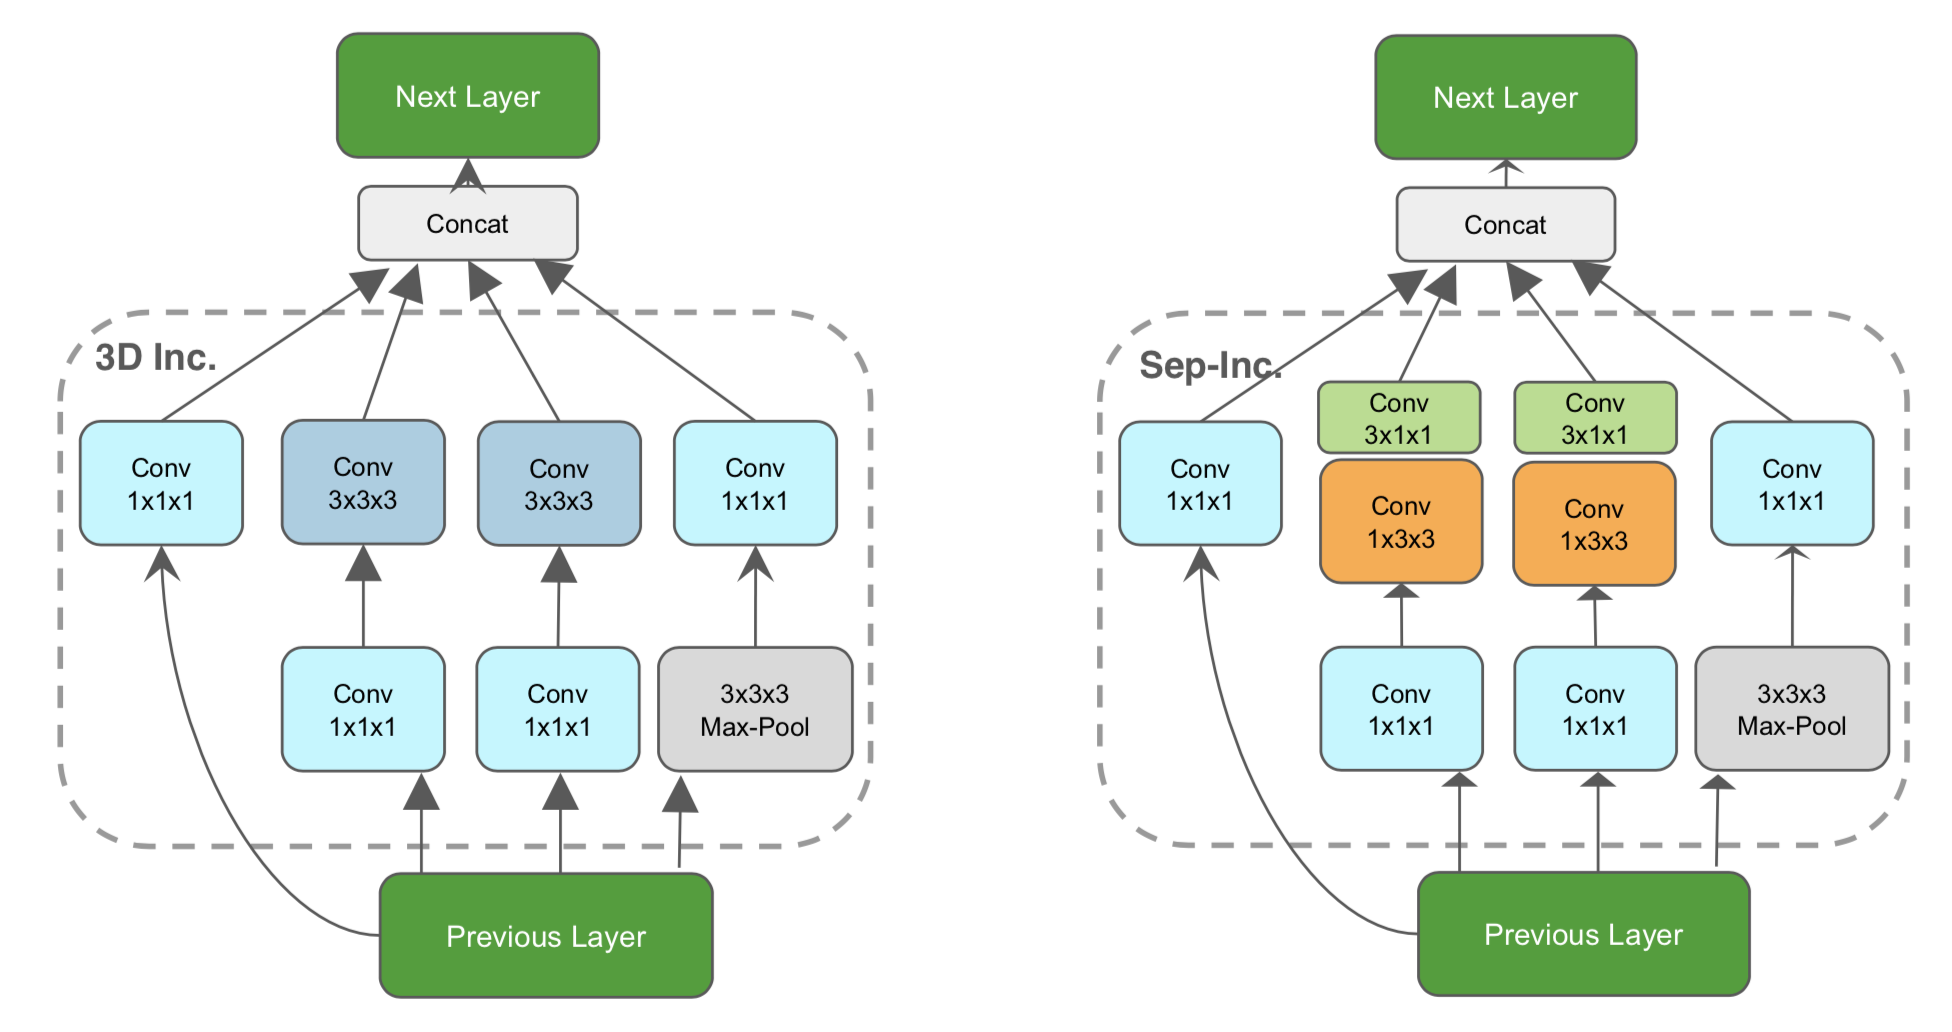
\includegraphics[width=0.35\textwidth]{figures/cv_deep_video_I3D.png}
		\caption{\textit{Left}: Standard Inception module of the I3D network. \textit{Right}: Inception module with 3D temporal separable convolutions.}
		\label{fig:deep_video_I3D_module}
	\end{figure}
	\item It is pretrained on ImageNet where the 2D filters are (after pretraining) inflated to a third dimension by repeating the values $N$ times over the time dimension, and rescaled by dividing by $N$
\end{itemize}
\subsubsection{Efficient 3D convolutions}
\begin{itemize}
	\item The main drawback of I3D and all other 3D convolutional networks are the huge amount of parameters. There are three ways to efficiently reduce the number of parameters
\end{itemize}
\begin{enumerate}
	\item \textbf{Pseudo 3D convolutions}
	\begin{itemize}
		\item The idea behind this operation is that the spatial and the temporal dimension do not correlate in every detail, but the temporal dimension is more important locally for the spatial dimension
		\item Thus, we split 3D convolution into a 2D spatial and a consecutive 1D temporal convolution. The concept is visualized in Figure~\ref{fig:deep_video_pseudo_3D_convs}
		\item The number of operations applied on input size $l_F \times w_F \times h_F \times c_F$ to output $l_G \times w_G \times h_G \times c_G$ is:
		\begin{equation*}
				\underbrace{k \times k \times 1 \times c_F \times c_I \times l_F \times w_G \times h_G}_{\text{Spatial 2D convolution}} + \underbrace{1\times 1\times k \times c_I \times c_G \times l_G \times w_G \times h_G}_{\text{Temporal 1D convolution}}
		\end{equation*}
		\item The speedup by this operation is about $\frac{1}{k}\cdot \frac{c_I}{c_G} \cdot \frac{l_F}{l_G} + \frac{1}{k^2} \cdot \frac{c_I}{c_F}\approx \frac{1}{k}\cdot \frac{c_I}{c_G}$
	\end{itemize}
	\begin{figure}[ht!]
		\centering
		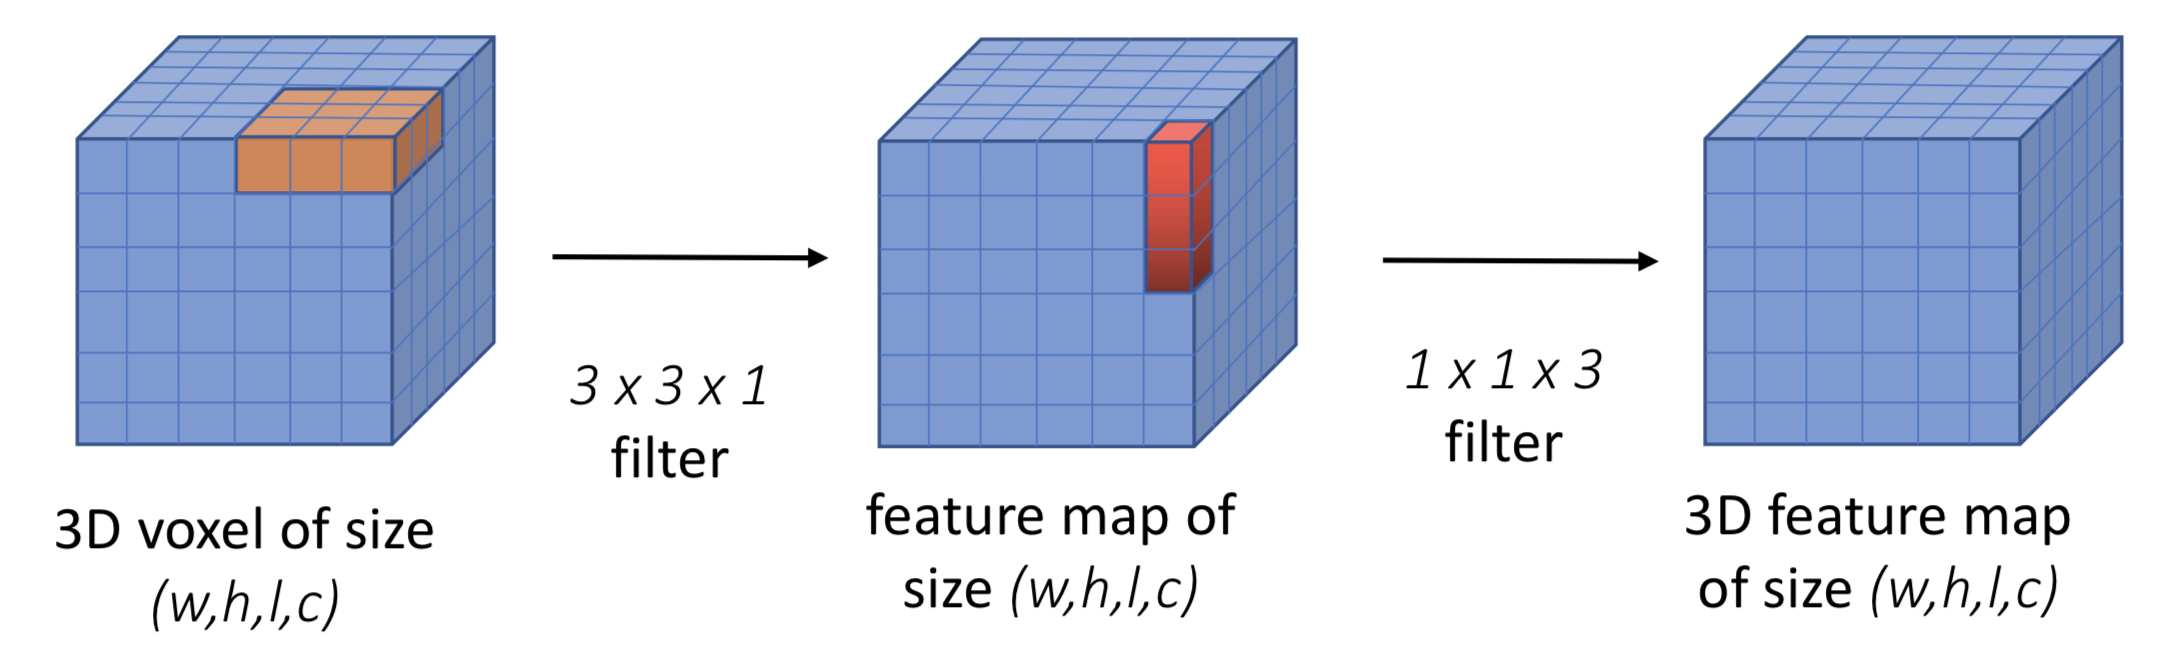
\includegraphics[width=0.55\textwidth]{figures/cv_deep_video_pseudo_3D_conv.png}
		\caption{Pseudo 3D convolutions split the operation into a spatial part (2D) and a temporal (1D) convolution.}
		\label{fig:deep_video_pseudo_3D_convs}
	\end{figure}
	\item \textbf{Depth-wise separable convolutions}
	\begin{itemize}
		\item This operation is inspired by the MobileNet architecture and removes the property of convolutions being depth-wise global
		\item We consider every input channel independently, and apply a different filter on each of them. For example, if we have an RGB input, we would apply three filters, each processing a different input channel
		\item To still allow interaction/combination of multiple channels, we apply a local $1\times 1\times 1$ convolution afterwards. Hence, an output channel depends again on all input channels.
		\item The number of operations applied on input size $l_F \times w_F \times h_F \times c_F$ to output $l_G \times w_G \times h_G \times c_G$ is:
		\begin{equation*}
			\underbrace{k \times k \times k \times 1 \times c_F \times l_G \times w_G \times h_G}_{\text{Depth-wise 3D convolution}} + \underbrace{1\times 1\times 1 \times c_F \times c_G \times l_G \times w_G \times h_G}_{\text{Local }1\times 1\times 1\text{ convolution}}
		\end{equation*}
		\item The speedup by this operation is considerably bigger than for pseudo 3D, namely $\frac{1}{c_G} + \frac{1}{k^{3}} \approx \frac{1}{k^{3}}$
		\begin{figure}[ht!]
			\centering
			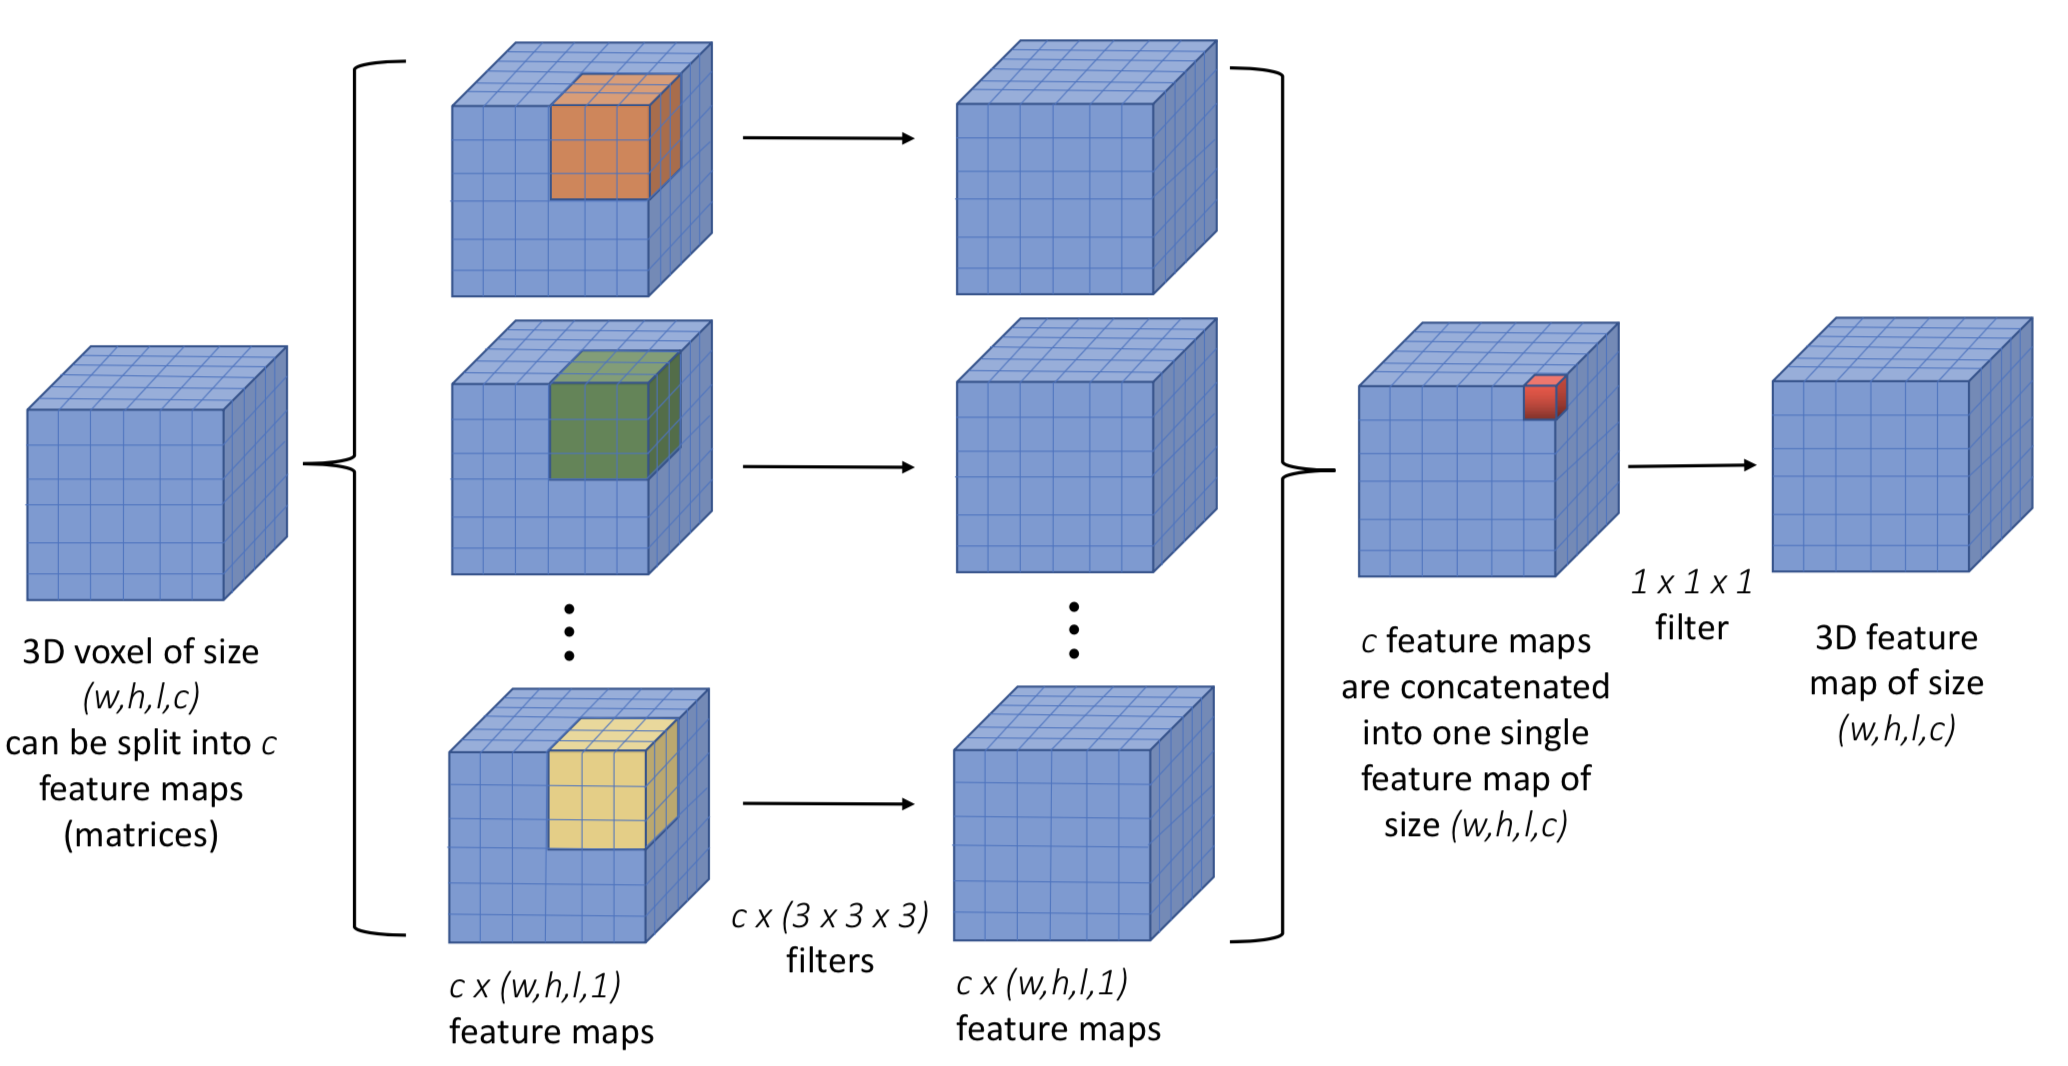
\includegraphics[width=0.6\textwidth]{figures/cv_deep_video_3D_depthwise_conv.png}
			\caption{Depth-wise 3D convolutions apply one filter per input channel, and combine the different channels afterwards. Same architecture is applied in MobileNet for the 2D case.}
			\label{fig:deep_video_depthwise_3D_convs}
		\end{figure}
	\end{itemize}
	\item \textbf{Partial 2D architecture} 
	\begin{itemize}
		\item Depending on the kind of motion we want to detect, it might not be necessary to apply 3D convolutions at every stage of the network. 
		\item For example, if we are only interested in high-level motions, we might want ot use a \textit{Top-heavy I3D} which applies 3D convolutions only on the last layers. 
		\item Similarly, for short motions, we might want to consider a \textit{Bottom-heavy I3D}. 
		\item Figure~\ref{fig:deep_video_I3D_architectures} summarizes the different network architectures.
		\begin{figure}[ht!]
			\centering
			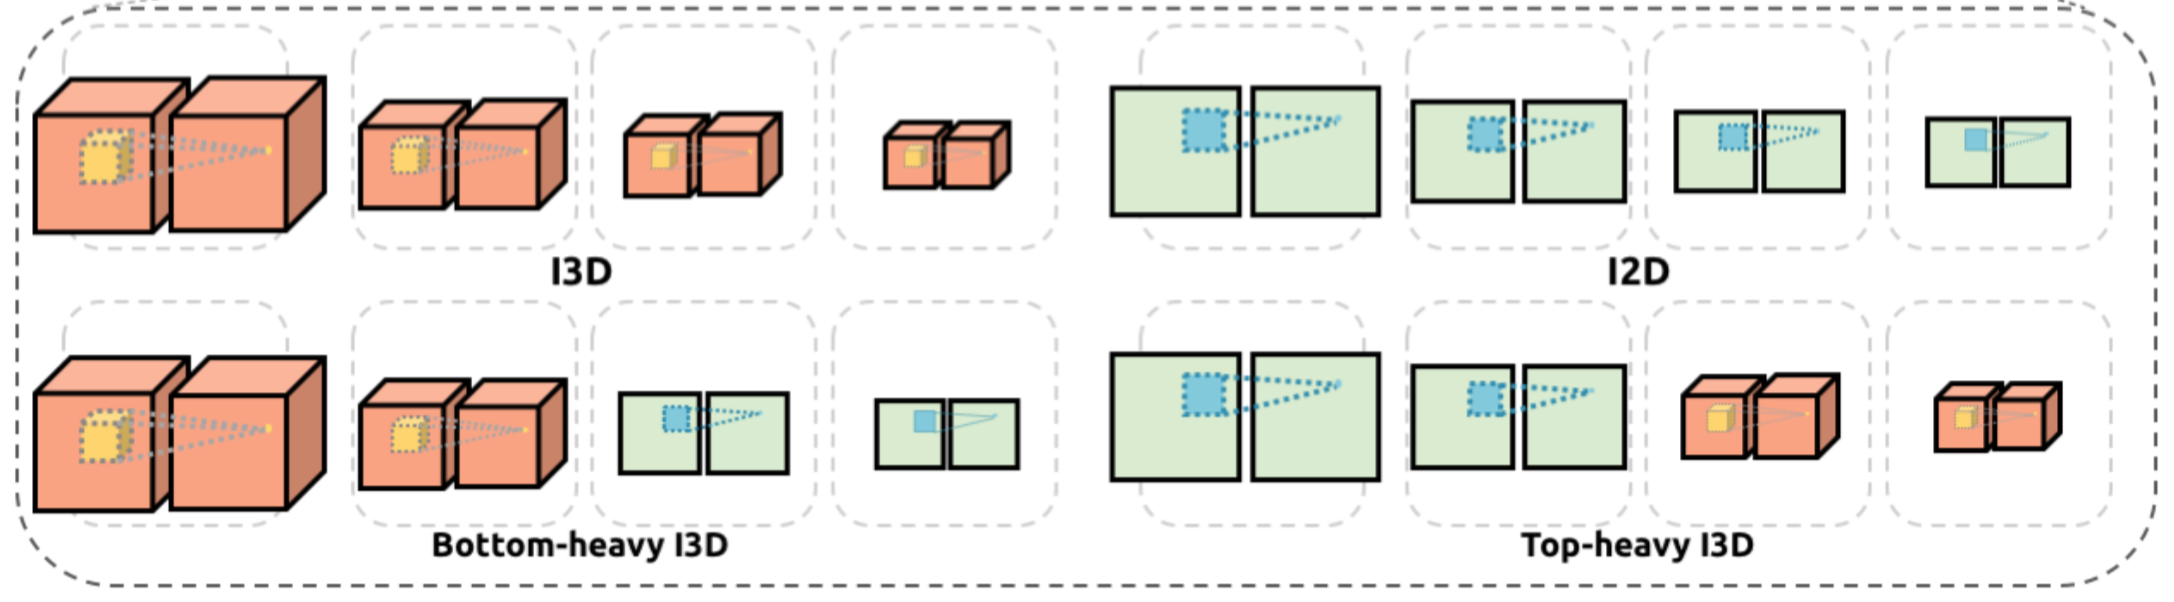
\includegraphics[width=0.6\textwidth]{figures/cv_deep_video_different_I3D_architectures.png}
			\caption{Different I3D network architectures.}
			\label{fig:deep_video_I3D_architectures}
		\end{figure}
	\end{itemize}
\end{enumerate}
\subsection{Self-supervised learning}
\begin{itemize}
	\item Learn to represent a video adequately in the network by using data and tasks where the labels are freely exploited. The great benefit is that we can use a lot of (unlabeled) data
	\item This is mostly done as a pre-training step as the network learns to deal and analyze with videos on a huge dataset. There are various tasks we can perform self-supervised learning on:
	\begin{itemize}
		\item \textbf{Visual tracking}: If we have given a tracking system, we can train a network to predict whether two patches are similar or not. Therefore, we create labels by the tracking system by setting it to 1 if two patches are the same object over time, or otherwise to 0 (we sample a random other patch from the image and compare the scores).
		\item \textbf{Learning by shuffling}: The network is given a set of frames, and its tasks is it to determine whether it is in the correct temporal order or not. The supervision signals are easily generated by labeling the real videos as positive, and shuffle their frame order to create a negative example. The goal is that the network learns to understand poses and motions over frames.
		\item \textbf{Learning by arrow of time}: The task of the network is to predict whether a video is played forwards of backwards (binary classification). This is a very challenging task as it requires the network to understand laws of physics (water only flows downwards, not upwards) by analyzing different motions in the video. One can cluster afterwards what clues the network had extracted which lead to a prediction of forward or backward (called \textit{arrow of time}). This approach gave the best self-supervised pre-training results so far, but is still not able to beat a supervised ImageNet pre-training.   
	\end{itemize}
\end{itemize}
\section{Applications}
Not in the exam :-)
\appendix
\newpage
\section{Practicals}
Gathering some interesting/important questions from the practicals and old exams.
\subsection{Color spaces}
\subsubsection{General parameters in color spaces}
\begin{itemize}
	\item \textbf{Chromaticity}: the color component regardless of its luminance/intensity. For example, the $xy$-diagram in Figure~\ref{fig:rgb_color_wavelength_distribution_XYZ_diagram} visualizes the chromaticity (includes saturation and hue)
	\item \textbf{Saturation}: defined as ``colorfulness of a stimulus relative to its own brightness''. In the normalized $rgb$ space, it is the distance to the point $(1/3,1/3,1/3)$ (ratio to the maximum distance). In case of the wavelength distribution, a color is saturated if it is very peaked.
	\item \textbf{Intensity}: the energy of the light. It is the integral of the wavelength distribution.
	\begin{figure}[ht!]
		\centering
		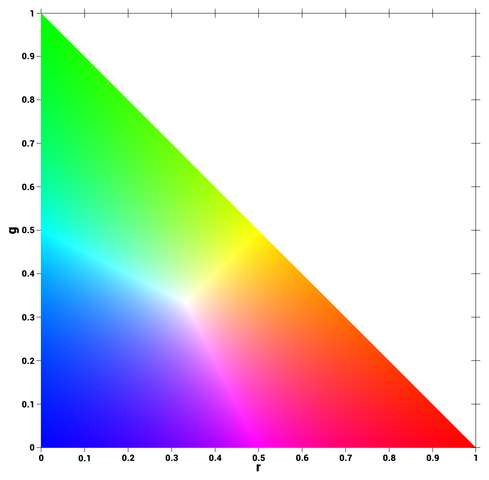
\includegraphics[width=0.25\textwidth]{figures/cv_image_formation_rg_chromaticity.png}
		\caption{\textit{rg}-chromaticity diagram. A point in this space symbolizes the chromaticity (color without intensity), and the distance to the point $(1/3,1/3)$ (if considered white light source as reference) with ratio to distance to border the saturation.}
	\end{figure}
\end{itemize}
\subsubsection{XYZ color space}
Calculate saturation, hue, intensity, plotting in the diagram, using reference lights, etc.

Interpolate between colors. We can perceive color (e.g. white) although it is not as we would define 
\subsubsection{Color invariance}
How to determine whether formula is color invariant or not. 
\begin{itemize}
	\item Color invariance is trying to remove transformations that do not directly affect the color, but let the sensor perceive it differently. 
	\item Hence, color invariant models are more or less insensitive to varying imaging conditions such as variations in illumination (light source) and object pose (shading, highlighting cues)
	\item For example, if we assume a Lambertian world where we only have body reflection and a white light source (equal for all wavelengths), we get for the $rgb$ space (note that $R=cos\theta \cdot e\cdot \int_{\lambda} p(\lambda) f_R(\lambda)d\lambda$):
	\begin{equation*}
		\begin{split}
			r & = \frac{R}{R + G + B} = \frac{\cancel{cos\theta} \cdot \cancel{e}\cdot \int_{\lambda} p(\lambda) f_R(\lambda)d\lambda}{\cancel{cos\theta} \cdot \cancel{e}\cdot \int_{\lambda} p(\lambda) \left(f_R(\lambda) + f_G(\lambda) + f_B(\lambda)\right)d\lambda}
		\end{split}
	\end{equation*}
	Thus, the \textit{rgb} color space is color invariant when assuming a Lambertian reflection model.
\end{itemize}
\subsection{Convolution operator}
\subsubsection{Difference between convolution and correlation}
Formally, correlation is a measurement of similarity between two signals whilst convolution is a measures the effect of one signal on the other. In practice however, correlation simply moves the filter over the image and computes the sum of the box at each pixel. Convolution is practically the same however before moving over the image, the filter is rotated 180 degrees. The formulas are:
\begin{equation*}
	\begin{split}
		\text{Correlation:} & I_{out} = I \otimes h,\hspace{1mm} I_{out}(i,j) = \sum\limits_{k,l} I(i+k, j+l) \cdot h(k,l)\\
		\text{Convolution:} &  I_{out} = I \ast h,\hspace{1mm} I_{out}(i,j) = \sum\limits_{k,l} I(i-k, j-l) \cdot h(k,l)
	\end{split}
\end{equation*}
Note that for both methods there is no difference in the result if we take the center pixel or a corner pixel as the start point for a filter. 
\subsubsection{Convolving two filters}
Two consecutive filters applied to an image can be summarized into one by convolving two filters. There are two ways to calculate the convolution of two filters. The more intuitive way to calculate the effect of every element of the second filter based on the first one.
Example:
\begin{equation*}
	\begin{split}
		f &=\left[\begin{array}{ccc}3 & 7 & 6\end{array}\right], \hspace{2mm}g=\left[\begin{array}{ccc}-1 & 5 & 8\end{array}\right] \Rightarrow f\ast g \\[5pt]
		& \implies \begin{array}{cccccc}
			& [-1\cdot 3 & 5\cdot 3 & 8\cdot 3] & & \\
		 +	& & [-1\cdot 7 & 5\cdot 7 & 8\cdot 7] & \\
		 +	& & & [-1\cdot 6 & 5\cdot 6 & 8\cdot 6] \\[5pt]
		 \hline
		 & [ -3 & 8 & 53 & 86 & 48 ]
		\end{array}
	\end{split}
\end{equation*}
The second option is to apply convolution right away with extended zero padding. We can imagine to use infinite zero padding but remove the zero elements in the convolved filter again. Note that we perform convolution, and therefore have to flip the second filter.
\begin{equation*}
	\begin{split}
		f\ast g & = \left[\begin{array}{ccccccc}0 & 0 & 3 & 7 & 6 & 0 & 0\end{array}\right] \otimes \left[\begin{array}{ccc}8 & 5 & -1\end{array}\right]\\
		& = \left[\begin{array}{ccccccc}-1\cdot 3 & (5\cdot 3 - 1\cdot 7) & (8\cdot 3 + 5\cdot 7 - 1\cdot 6) & (8\cdot 7 + 5\cdot 6) & 8\cdot 6\end{array}\right]\\
		& = \left[\begin{array}{ccccc}-3 & 8 & 53 & 86 & 48\end{array}\right]
	\end{split}
\end{equation*}
\subsubsection{Linearly Separable Filters}
Some 2D filters are separable in their $x$ and $y$ dimension. We can test it by comparing the convolution of separated $x$ and $y$ filters with the 2D version.
\begin{itemize}
	\item \textit{What is the benefit of separable filters?}
	
	\underline{Answer}: The computational cost is reduced form $k^2$ to $2\cdot k$.
	
	\item \textit{Prove that a 2D Gaussian filter is linearly separable.}
	
	\underline{Answer}: We can show this holds for the continuous case, and thus also for the discrete. Note that we can neglect a constant factor $c$ for normalization as this does not introduce any significant computational effort.
	\begin{equation*}
		\begin{split}
			G_x * G_y  & = \frac{1}{\sqrt{2\pi}\sigma} e^{-\frac{x^2}{2\sigma^2}} * \frac{1}{\sqrt{2\pi}\sigma} e^{-\frac{y^2}{2\sigma^2}}\\
			& = \frac{1}{2\pi\sigma^2} e^{-\frac{x^2 + y^2}{2\sigma^2}}\\
			& = G_{xy}
		\end{split}
	\end{equation*}
	\item \textit{Prove that a 2D box filter (size $3\times 3$) is linearly separable.}
	
	\underline{Answer}: We can show this by simply computing the convolution.
	\begin{equation*}
	\begin{split}
		\left[\begin{array}{ccc}1 & 1 & 1\end{array}\right] *  
		\left[\begin{array}{c}1 \\ 1 \\ 1\end{array}\right] & = \left[\begin{array}{ccc}
		1 & 1 & 1\\ 1 & 1 & 1\\ 1 & 1 & 1
		\end{array}\right]\\
	\end{split}
	\end{equation*}
	\item \textit{Check whether the following 2D filter is linearly separable:}
	$$h = \left[\begin{array}{ccc}
	1 & -2 & 1\\ -2 & 4 & -2\\ 1 & -2 & 1
	\end{array}\right]$$
	
	\underline{Answer}: The way to check that is looking for symmetric patterns in $x$ and $y$ direction which are independent of the other dimension. In this case, we can easily spot the pattern:
	\begin{equation*}
	\begin{split}
	\left[\begin{array}{ccc}1 & -2 & 1\end{array}\right] *  
	\left[\begin{array}{c}1 \\ -2 \\ 1\end{array}\right] & = \left[\begin{array}{ccc}
	1 & -2 & 1\\ -2 & 4 & -2\\ 1 & -2 & 1
	\end{array}\right]\\
	\end{split}
	\end{equation*}
	\item \textit{Check whether the following 2D filter is linearly separable:}
	$$h = \left[\begin{array}{ccc}
	1 & 8 & 3\\ 7 & 6 & 2\\ 4 & 9 & 5
	\end{array}\right]$$
	
	\underline{Answer}:  No, this kernel is not linearly separable.
\end{itemize}
\subsection{Object detection}

\subsection{Convolutional Neural Networks}
\subsubsection{Amount of parameters, output size and computational cost}
\begin{itemize}
	\item \textbf{Output size}: the spatial output size of a convolutional layer depends on the kernel size $k$, the padding $p$ (per side), the stride $s$ and the input size $w_i$. The output size is then calculated by $w_o = (w_i + 2\cdot p - k)/s + 1$
	\begin{itemize}
		\item \textit{What is the size of the output volume with stride $3$, kernel $5\times 5$, number of neurons $5$ and input size $32\times 32\times 3$ (no padding)?}
		
		\underline{Answer}: The output size is $w_0 = (32 + 2\cdot 0 - 5)/3 + 1 = 10$.
		
		\item \textit{What padding size is required to keep the output size equals to the input size for a kernel $k$ and stride $s$?}
		
		\underline{Answer}: we have to reverse the equation above to:
		\begin{equation*}
			\begin{split}
				w_o = w_i & = (w_i + 2\cdot p - k)/s + 1\\
				\Leftrightarrow (w_i - 1) \cdot s & = w_i + 2\cdot p - k\\
				\Leftrightarrow p & = \frac{1}{2}\left(w_i \cdot \left(s-1\right) - s + k\right)
			\end{split}
		\end{equation*}
		Hence, if stride is $s=1$, the necessary padding is $p=\frac{k-1}{2}$.
		
		\item \textit{How many output frames do we get for a 3D convolution of $3\times 3\times 3$ (stride $s=3$ and padding $p=1$ in temporal dimension) on a input video size of $16\times 256\times 256\times 3$?}
		
		\underline{Answer}: We can apply the same formula as before: $l_o = (16 + 2\cdot 1 - 3)/3 + 1 = 6$ output frames.
	\end{itemize}
	\item \textbf{Number of parameters}: a 2D convolution contains $k\times k\times c_F \times c_G$ parameters where $k$ is the kernel size, and $c_F$ and $c_G$ the number of input and output channels. For a 3D convolution, we multiply it by another $k$. Note that all these three $k$'s can be different (e.g. $3\times 3\times 1$, $5\times 1 \times 1$, ...)
	\begin{itemize}
		\item \textit{How many parameters are learned in a convolutional layer with an RGB input image, $5\times 5$ kernel size and $100$ different filters?}
		
		\underline{Answer}: We learn $5\times 5\times 3\times 100 = 7,500$ parameters for the filters, and $100$ biases. Thus, we have overall $7,600$ parameters.
		
		\item \textit{How many parameters are learned if we set the padding to $p=2$ and stride $s=2$?}

		\underline{Answer}: The number of parameters is independent of the stride and the padding.
	\end{itemize}
	\item \textbf{Computational cost}: The computational cost of a layer is the cost of a single filter application (the filter size) times the number of output neurons.
	\begin{itemize}
		\item \textit{Given the input $w_F \times h_F \times c_F$ and output $w_G \times h_G \times c_G$, what is the computational cost of a 2D convolution with kernel size $k\times k$ between these two layers?}
		
		\underline{Answer}: The cost of applying a single filter once is $k\times k\times c_F$. We then have to move the filter over $x$ and $y$ dimension, and repeat it for $c_G$ filters. Thus, the overall cost is determined by:
		$$k\times k\times c_F\times c_G\times w_G\times h_G$$
		
		\item \textit{Given the input $256 \times 256 \times 3$, what is the computational cost of a 2D convolution with kernel size $7\times 7$, $32$ output channels, stride $s=3$ and padding $p=0$?}
		
		\underline{Answer}: We first have to calculate the output size $w_G = (w_F + 2\cdot p - k)/s + 1 = (256 + 0 - 7)/3 = 83$ and $h_G = 83$. Next, we can apply our previous formula:
		$7\times 7\times 3\times 32\times 83\times 83$
		
		\item \textit{What are two ways to reduce the number of computations for 2D convolutions?}
		
		\underline{Answer}: Same as in case of 3D convolutions. We can either do depth-wise convolutions (\textit{MobileNet}), or do pseudo 2D convolutions by separating the filter $k\times k$ to a $1\times k$ and $k\times 1$ convolution (\textit{InceptionV2}).
	\end{itemize}
\end{itemize}
\subsubsection{Other general questions}
\begin{itemize}
	\item \textbf{Locally constrained layer}: A convolutional layer where we don't share weights over spatial dimensions.
	\begin{itemize}
		\item \textit{How many parameters are needed for a locally constrained layer, where each neuron looks at a $10\times10$ window, when using $W=H=100$, and stride of $5$?}
		
		\underline{Answer}: The spatial output size is $(100 - 10) / 5 + 1 = 19$ so that we have $19\times 19=361$ different kernels. Combined with the kernel/window size, we get overall $10\times 10\times 361=36,100$ parameters.
		\item \textit{Describe a scenario where weight sharing as done in plain convolutional layers is not beneficial for recognition}
		
		\underline{Answer}: Weight sharing works most effectively, if the input is transitional invariant. However, if this is not the case and we have stationary data, we should for example use locally constrained layers where the weights are not shared. This may lead to more parameters but reduces the required amount of channels (restricted number of possible objects per position). Example: face recognition with standardized position (eyes and mouth filters at different parts of the image). 
	\end{itemize}
\end{itemize}

\end{document}